\documentclass{beamer}
\usepackage[utf8]{inputenc}
\usepackage{graphicx, epsfig}
\usepackage{amsmath,mathrsfs,amsfonts,amssymb}
\usepackage{floatflt}
\usepackage{epic,ecltree}
\usepackage{mathtext}
\usepackage{fancybox}
\usepackage{fancyhdr}
\usepackage{multirow}
\usepackage{enumerate}
\usepackage{epstopdf}
\usepackage{multicol}
\usepackage{algorithm}
\usepackage[noend]{algorithmic}
\usepackage{tikz}
\usepackage{blindtext}
\usetheme{default}%{Singapore}%{Warsaw}%{Warsaw}%{Darmstadt}
\usecolortheme{default}

\setbeamerfont{title}{size=\Huge}
\setbeamertemplate{footline}[page number]{}

\setbeamertemplate{section in toc}[sections numbered]


\makeatletter
\newcommand\HUGE{\@setfontsize\Huge{35}{40}}
\makeatother    

\setbeamerfont{title}{size=\HUGE}
\beamertemplatenavigationsymbolsempty

% latin bold lower
\newcommand{\ba}{\mathbf{a}} 
\newcommand{\bc}{\mathbf{c}} 
\newcommand{\be}{\mathbf{e}} 
\newcommand{\bff}{\mathbf{f}} % \bf - for bold type
\newcommand{\bg}{\mathbf{g}} 
\newcommand{\bh}{\mathbf{h}} 
\newcommand{\bp}{\mathbf{p}} 
\newcommand{\bq}{\mathbf{q}} 
\newcommand{\bt}{\mathbf{t}} 
\newcommand{\bs}{\mathbf{s}} 
\newcommand{\bu}{\mathbf{u}} 
\newcommand{\bv}{\mathbf{v}} 
\newcommand{\bw}{\mathbf{w}} 
\newcommand{\bx}{\mathbf{x}} 
\newcommand{\by}{\mathbf{y}} 
\newcommand{\bz}{\mathbf{z}} 

% latin bold upper
\newcommand{\bA}{\mathbf{A}} 
\newcommand{\bB}{\mathbf{B}} 
\newcommand{\bC}{\mathbf{C}} 
\newcommand{\bG}{\mathbf{G}} 
\newcommand{\bI}{\mathbf{I}} 
\newcommand{\bJ}{\mathbf{J}} 
\newcommand{\bL}{\mathbf{L}} 
\newcommand{\bM}{\mathbf{M}} 
\newcommand{\bP}{\mathbf{P}}
\newcommand{\bQ}{\mathbf{Q}} 
\newcommand{\bR}{\mathbf{R}} 
\newcommand{\bT}{\mathbf{T}} 
\newcommand{\bU}{\mathbf{U}} 
\newcommand{\bV}{\mathbf{V}} 
\newcommand{\bW}{\mathbf{W}} 
\newcommand{\bX}{\mathbf{X}} 
\newcommand{\bY}{\mathbf{Y}} 
\newcommand{\bZ}{\mathbf{Z}} 

% latin cal upper
\newcommand{\cF}{\mathcal{F}} 
\newcommand{\cG}{\mathcal{G}} 
\newcommand{\cI}{\mathcal{I}} 
\newcommand{\cL}{\mathcal{L}} 
\newcommand{\cM}{\mathcal{M}} 
\newcommand{\cN}{\mathcal{N}} 
\newcommand{\cP}{\mathcal{P}} 
\newcommand{\cS}{\mathcal{S}} 
\newcommand{\cT}{\mathcal{T}} 
\newcommand{\cW}{\mathcal{W}} 
\newcommand{\cX}{\mathcal{X}} 
\newcommand{\cZ}{\mathcal{Z}} 

% latin bb upper
\newcommand{\bbE}{\mathbb{E}} 
\newcommand{\bbI}{\mathbb{I}} 
\newcommand{\bbP}{\mathbb{P}} 
\newcommand{\bbR}{\mathbb{R}} 

% greek bold lower
\newcommand{\bepsilon}{\boldsymbol{\epsilon}} 
\newcommand{\btheta}{\boldsymbol{\theta}} 
\newcommand{\blambda}{\boldsymbol{\lambda}} 
\newcommand{\bpi}{\boldsymbol{\pi}} 
\newcommand{\bmu}{\boldsymbol{\mu}} 
\newcommand{\bsigma}{\boldsymbol{\sigma}} 
\newcommand{\bphi}{\boldsymbol{\phi}} 

% greek bold upper
\newcommand{\bSigma}{\boldsymbol{\Sigma}} 

\DeclareMathOperator*{\argmin}{arg\,min}
\DeclareMathOperator*{\argmax}{arg\,max}

\newcommand{\createdgmtitle}[1]{\title[\hbox to 56mm{Deep Generative Models  \hfill\insertframenumber\,/\,\inserttotalframenumber}]
	{\vspace{1cm} \\ \textbf{Deep Generative Models} \\ {\Huge Lecture #1}}
	\author{Roman Isachenko}
		\institute{
\includegraphics[width=0.7cm]{../utils/aimasterslogo} \LARGE{AI Masters}}
	\date{2024, Spring}
}

\usepackage{tikz}
\usetikzlibrary{arrows,shapes,positioning,shadows,trees}

\newcommand\myfootnote[1]{%
  \tikz[remember picture,overlay]
  \draw (current page.south west) +(1in + \oddsidemargin,0.5em)
  node[anchor=south west,inner sep=0pt]{\parbox{\textwidth}{%
      \rlap{\rule{10em}{0.4pt}}\raggedright\scriptsize \textit{#1}}};}

\newcommand\myfootnotewithlink[2]{%
  \tikz[remember picture,overlay]
  \draw (current page.south west) +(1in + \oddsidemargin,0.5em)
  node[anchor=south west,inner sep=0pt]{\parbox{\textwidth}{%
      \rlap{\rule{10em}{0.4pt}}\raggedright\scriptsize\href{#1}{\textit{#2}}}};}
      
\AtBeginSection[]
      {
      	\begin{frame}{Outline}
      		\tableofcontents[currentsection]
      	\end{frame}
      }
      \AtBeginSubsection[]{
      	\begin{frame}{Outline}
      		\tableofcontents[currentsection,currentsubsection]
      	\end{frame}
}
\createdgmtitle{14}

\usepackage{tikz}

\usetikzlibrary{arrows,shapes,positioning,shadows,trees}
%--------------------------------------------------------------------------------
\begin{document}
%--------------------------------------------------------------------------------
\begin{frame}[noframenumbering,plain]
%\thispagestyle{empty}
\titlepage
\end{frame}
%=======
\begin{frame}{Outline}
	\tableofcontents
\end{frame}
%=======
%=======
\begin{frame}{Recap of previous lecture}
	\begin{block}{Discrete-in-time objective}
		\vspace{-0.3cm}
		\[
			\bbE_{\pi(\bx_0)} \bbE_{t \sim U\{1, T\}} \bbE_{q(\bx_t | \bx_0)}\bigl\| \bs_{\btheta, t}(\bx_t) - \nabla_{\bx_t} \log q(\bx_t | \bx_0) \bigr\|^2_2 
		\]
		\vspace{-0.5cm}
	\end{block}
	\begin{block}{Continuous-in-time objective}
		\vspace{-0.5cm}
		\[
			\bbE_{\pi(\bx(0))} \bbE_{t \sim U[0, 1]} \bbE_{q(\bx(t) | \bx(0))}\bigl\| \bs_{\btheta}(\bx(t), t) - {\color{teal}\nabla_{\bx(t)} \log q(\bx(t) | \bx(0))} \bigr\|^2_2 
		\]
		\vspace{-0.5cm}
	\end{block}
	\begin{block}{NCSN}
		\vspace{-0.3cm}
		\[
			q(\bx(t) | \bx(0)) = \cN\left(\bx(0), \left[\sigma^2(t) - \sigma^2(0)\right] \cdot \bI\right)
		\]
		\vspace{-0.5cm}
	\end{block}
	\begin{block}{DDPM}
		\vspace{-0.3cm}
		\[
			q(\bx(t) | \bx(0)) = \cN\left(\bx(0) e^{-\frac{1}{2} \int_0^t\beta(s)ds}, \left(1 - e^{- \int_0^t\beta(s)ds}\right) \cdot \bI\right)
		\]
		\vspace{-0.5cm}
	\end{block}
	
	\myfootnotewithlink{https://arxiv.org/abs/2011.13456}{Song Y., et al. Score-Based Generative Modeling through Stochastic Differential Equations, 2020}
\end{frame}
%=======
\begin{frame}{Recap of previous lecture}
	\begin{block}{Sampling}
		Solve reverse SDE using numerical solvers (SDESolve).
		\begin{figure}
			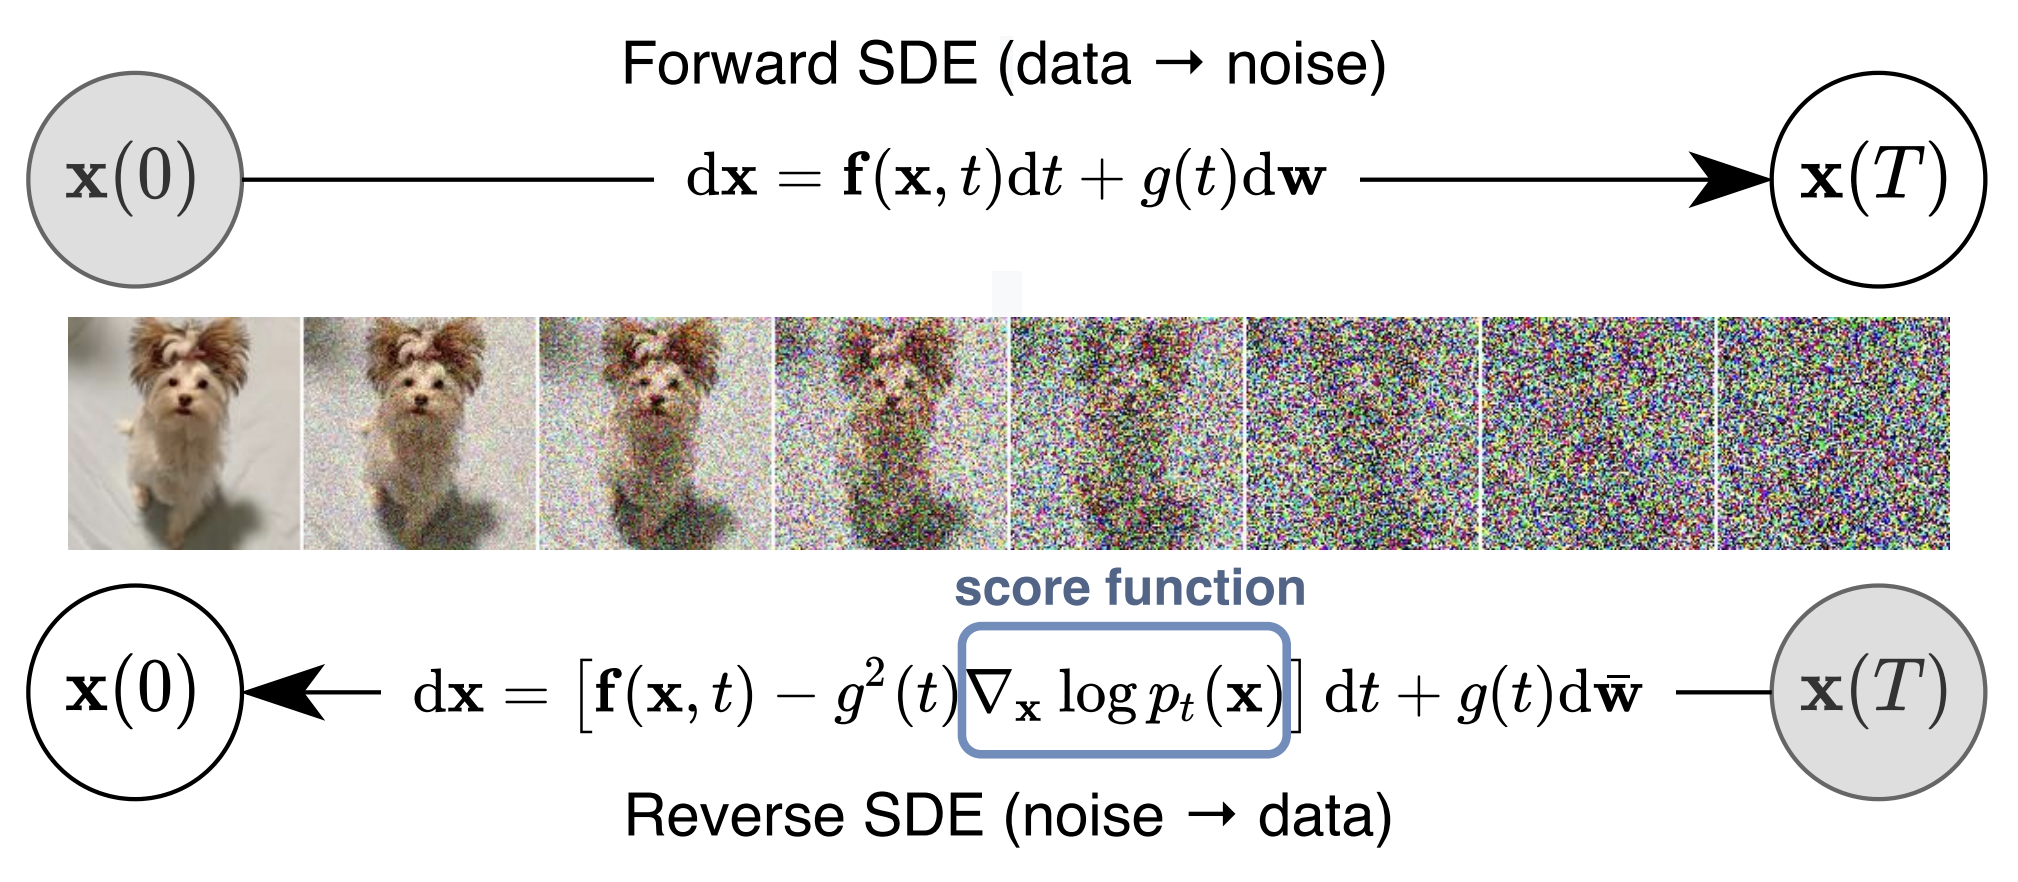
\includegraphics[width=0.8\linewidth]{figs/sbgm}
		\end{figure}
		\vspace{-0.5cm}
	\end{block}
	\begin{itemize}
		\item Discretization of the reverse SDE gives us the ancestral sampling.
		\item If we use probability flow instead of SDE than the reverse ODE gives us the DDIM sampling.
	\end{itemize}
	\myfootnotewithlink{https://arxiv.org/abs/2011.13456}{Song Y., et al. Score-Based Generative Modeling through Stochastic Differential Equations, 2020}
\end{frame}
%=======
\begin{frame}{Recap of previous lecture}
	Let consider ODE dynamic $\bx(t)$ in time interval $t \in [0, 1]$ with $\bx_0 \sim p_0(\bx) = p(\bx)$, $\bx_1 \sim p_1(\bx) =  \pi(\bx)$.
	\[
		\frac{d \bx}{dt} = \bff (\bx, t),  \quad \text{with initial condition }\bx(0) = \bx_0.
	\]
	\vspace{-0.5cm}
	\begin{block}{KFP theorem (continuity equation)}
		\vspace{-0.5cm}
		\[
			\frac{\partial p_t(\bx)}{\partial t} = - \text{div}\left(\bff(\bx, t) p_t(\bx)\right) \Leftrightarrow \frac{d \log p_t(\bx(t))}{d t} = - \text{tr} \left( \frac{\partial \bff(\bx(t), t)}{\partial \bx(t)} \right)
		\]
		\vspace{-0.3cm}
	\end{block}
	Solving the continuity equation using the adjoint method is complicated and unstable process.
	\begin{block}{Flow Matching}
		\vspace{-0.3cm}
		\[
			\bbE_{t \sim U[0, 1]} \bbE_{\bx \sim p_t(\bx)}\left\| \bff(\bx, t) - \bff_{\btheta}(\bx, t) \right\|^2 \rightarrow \min_{\btheta}
		\]
		\vspace{-0.3cm}
	\end{block}
	\myfootnotewithlink{https://arxiv.org/abs/2210.02747}{Lipman Y., et al. Flow Matching for Generative Modeling, 2022}
\end{frame}
%=======
\begin{frame}{Recap of previous lecture}
	\vspace{-0.3cm}
	Let introduce the latent variable $\bz$:
	\[
		p_t(\bx) = \int p_t(\bx | \bz) p(\bz) d \bz 
	\]
	\vspace{-0.5cm}
	\[
		\frac{\partial p_t(\bx | \bz)}{\partial t} = - \text{div}\left(\bff(\bx, \bz, t) p_t(\bx | \bz)\right).
	\]
	\vspace{-0.3cm}
	\begin{itemize}
		\item $p_t(\bx | \bz)$ is a \textbf{conditional probability path};
		\item $\bff(\bx, \bz, t)$ is a \textbf{conditional vector field}.
	\end{itemize}
	\[
		\frac{d\bx}{dt} = \bff(\bx, t) \quad \Rightarrow \quad \frac{d\bx}{dt} = \bff(\bx, \bz, t)
	\]
	\vspace{-0.5cm}
	\begin{block}{Theorem}
		The following vector field generates the probability path $p_t(\bx)$.
		\vspace{-0.2cm}
		\[
			\bff(\bx, t) = \bbE_{p_t(\bz | \bx)} \bff(\bx, \bz, t)  = {\color{teal}\int \bff(\bx, \bz, t)} \frac{\color{teal}p_t(\bx | \bz) p(\bz)}{p_t(\bx)} {\color{teal}d \bz}
		\]
		\vspace{-0.5cm}
	\end{block}
	\myfootnotewithlink{https://arxiv.org/abs/2302.00482}{Tong A., et al. Improving and Generalizing Flow-Based Generative Models with Minibatch Optimal Transport, 2023}
\end{frame}
%=======
\begin{frame}{Recap of previous lecture}
	\begin{block}{Flow Matching (FM)}
		\vspace{-0.5cm}
		\[
			\bbE_{t \sim U[0, 1]} \bbE_{\bx \sim p_t(\bx)}\left\| \bff(\bx, t) - \bff_{\btheta}(\bx, t) \right\|^2 \rightarrow \min_{\btheta}
		\]
		\vspace{-0.5cm}
	\end{block}
	\begin{block}{Conditional Flow Matching (CFM)}
		\vspace{-0.5cm}
		\[
			\bbE_{t \sim U[0, 1]} \bbE_{\bz \sim p(\bz)} \bbE_{\bx \sim p_t(\bx | \bz)}\left\| \bff(\bx, \bz, t) - \bff_{\btheta}(\bx, t) \right\|^2 \rightarrow \min_{\btheta}
		\]
		\vspace{-0.5cm}
	\end{block}
	\begin{block}{Theorem}
		If $\text{supp}(p_t(\bx)) = \bbR^m$, then the optimal value of FM objective is equal to the optimal value of CFM objective.
	\end{block}
	\begin{figure}
		\centering
		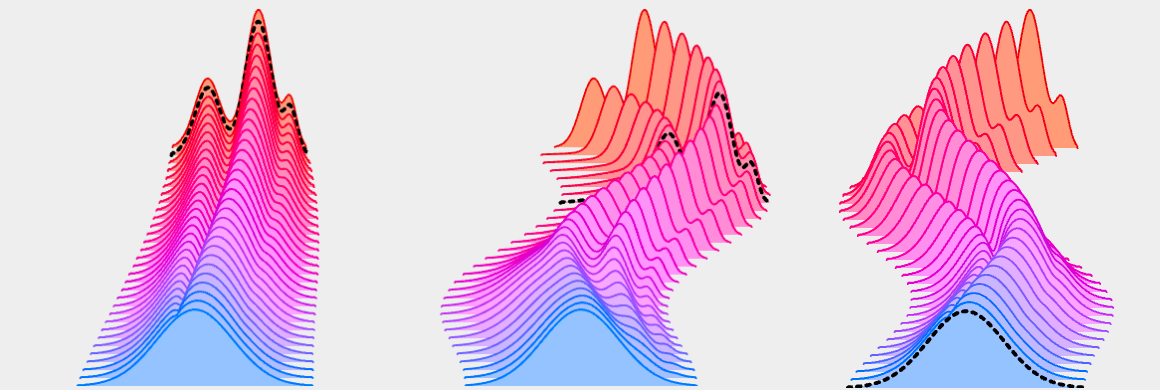
\includegraphics[width=0.8\linewidth]{figs/multiple_dynamics}
	\end{figure}
	\myfootnotewithlink{https://arxiv.org/abs/2302.00482}{Tong A., et al. Improving and Generalizing Flow-Based Generative Models with Minibatch Optimal Transport, 2023}
\end{frame}
%=======
\begin{frame}{Recap of previous lecture}
	\begin{figure}
		\centering
		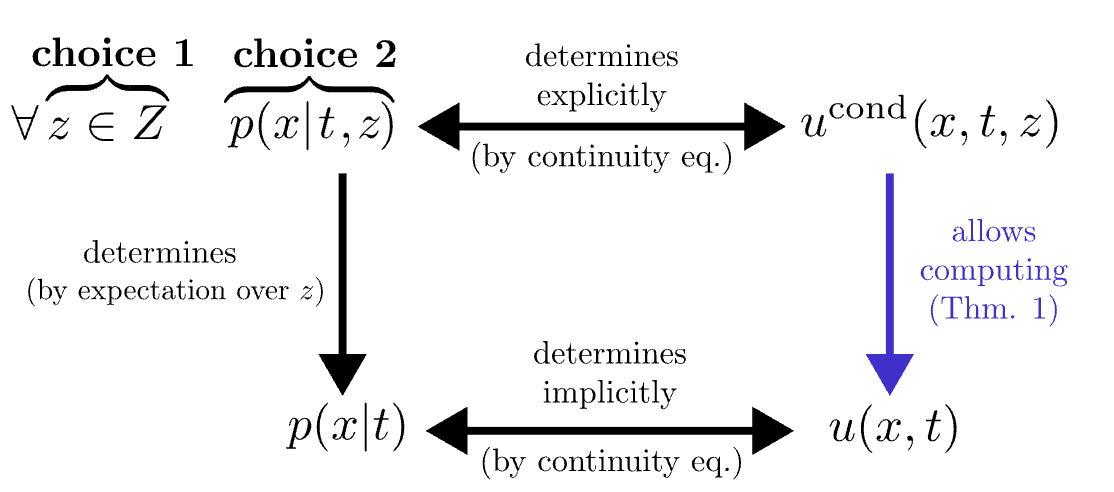
\includegraphics[width=0.7\linewidth]{figs/cfm_uncond_to_cond}
	\end{figure}
	\vspace{-0.3cm}
	\begin{block}{Constraints}
		\vspace{-0.3cm}
		\[
			p(\bx) = \cN(0, \bI) = \bbE_{p(\bz)} p_0(\bx | \bz); \quad \pi(\bx) = \bbE_{p(\bz)} p_1(\bx | \bz).
		\]
		\vspace{-0.5cm}
	\end{block}
	\begin{itemize}
		\item How to choose the conditioning latent variable $\bz$?
		\item How to define $p_t(\bx | \bz)$ which follows the constraints?
	\end{itemize}
	\begin{block}{Gaussian conditional probability path}
		\vspace{-0.3cm}
		\[
			p_t(\bx | \bz) = \cN\left(\bmu_t(\bz), \bsigma_t^2(\bz)\right)
		\]
		\[
			\bx_t = \bmu_t(\bz) + \bsigma_t(\bz) \odot \bx_0, \quad {\color{violet} \bx_0 \sim p_0(\bx) = \cN(0, \bI)}
		\]
	\end{block}
		\myfootnotewithlink{https://dl.heeere.com/conditional-flow-matching/blog/conditional-flow-matching}{image credit: A Visual Dive into Conditional Flow Matching}
\end{frame}
%=======
\begin{frame}{Recap of previous lecture}
	\begin{block}{Gaussian conditional probability path}
		\vspace{-0.3cm}
		\[
			p_t(\bx | \bz) = \cN\left(\bmu_t(\bz), \bsigma_t^2(\bz)\right); \quad \bx_t = \bmu_t(\bz) + \bsigma_t(\bz) \odot \bx_0
		\]
		\vspace{-0.3cm}
		\[
			\bff(\bx, \bz, t) =  \bmu_t'(\bz) + \frac{\bsigma_t'(\bz)}{\bsigma_t(\bz)} \odot (\bx - \bmu_t(\bz))
		\]
		\vspace{-0.3cm}
	\end{block}
	\begin{block}{Conditioning latent variable}
		Let choose $\bz = \bx_1$. Then $p(\bz) = p_1(\bx_1)$.
		\[
			p_t(\bx) = \int p_t(\bx | \bx_1) p_1(\bx_1) d \bx_1
		\]
		\vspace{-0.5cm}
	\end{block}
	We need to ensure boundary constraints:
	\[
		\begin{cases}
			p(\bx) = \bbE_{p(\bz)} p_0(\bx | \bz); {\color{gray}(= \cN(0, \bI))} \\
			\pi(\bx) = \bbE_{p(\bz)} p_1(\bx | \bz).
		\end{cases}
		\quad \Rightarrow \quad 
		\begin{cases}
			p_0(\bx | \bx_1) = \cN(0, \bI); \\
			p_1(\bx | \bx_1) = \delta(\bx - \bx_1).
		\end{cases}
	\]
	\vspace{-0.3cm}
	\myfootnotewithlink{https://arxiv.org/abs/2210.02747}{Lipman Y., et al. Flow Matching for Generative Modeling, 2022}
\end{frame}
%=======
\begin{frame}{Recap of previous lecture}
	\[
		p_0(\bx | \bx_1) = \cN(0, \bI); \quad p_1(\bx | \bx_1) = \delta(\bx - \bx_1).
	\]
	
	\begin{block}{Gaussian conditional probability path}
		\vspace{-0.5cm}
		\[
			p_t(\bx | \bx_1) = \cN\left(\bmu_t(\bx_1), \bsigma_t^2(\bx_1)\right); \quad \bx_t = \bmu_t(\bx_1) +  \bsigma_t^2(\bx_1) \odot \bx_0.
		\]
		\vspace{-0.6cm}
	\end{block}
	Let consider straight conditional paths	
	\[
		\begin{cases}
			\bmu_t(\bx_1) = t \bx_1; \\
			\bsigma_t(\bx_1) = (1 - t).
		\end{cases}
		\quad \Rightarrow \quad 
		\begin{cases}
			p_t(\bx | \bx_1) = \cN\left(t \bx_1, (1-t)^2 \bI\right); \\
		 	\bx_t = t \bx_1 + (1 - t) \bx_0. 
	 \end{cases}
	\]
	\vspace{-0.3cm}
	\begin{figure}
		\centering
		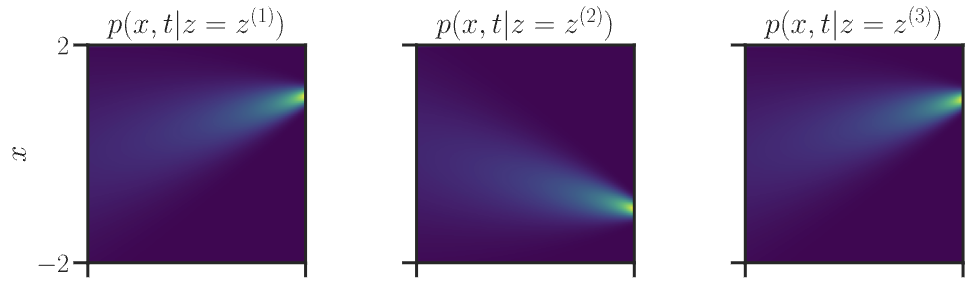
\includegraphics[width=\linewidth]{figs/conical_paths}
	\end{figure}
	\myfootnotewithlink{https://dl.heeere.com/conditional-flow-matching/blog/conditional-flow-matching}{image credit: A Visual Dive into Conditional Flow Matching}
\end{frame}
%=======
\section{Conditional flow matching}
%=======
\subsection{Conical gaussian paths (continued)}
%=======
\begin{frame}{Conical gaussian paths}
	\vspace{-0.3cm}
	\[
		p_t(\bx | \bx_1) = \cN\left(t \bx_1, (1-t)^2 \bI\right); \quad {\color{teal}\bx_t = t \bx_1 + (1 - t) \bx_0}. 
	\]
	\vspace{-0.5cm}
	\begin{block}{Conditional vector field}
		\vspace{-0.3cm}
		\[
			 \frac{d\bx}{dt} = \bff(\bx, \bx_1, t) =  \bmu_t'(\bx_1) + \frac{\bsigma_t'(\bx_1)}{\bsigma_t(\bx_1)} \odot (\bx - \bmu_t(\bx_1))
		\]
		\vspace{-0.5cm}
		\begin{multline*}
			\bff(\bx, \bx_1, t) = \bx_1 - \frac{1}{1-t} \cdot (\bx - t \bx_1) = \frac{\bx_1 - {\color{teal}\bx}}{1-t} = \\
			= \frac{\bx_1 - {\color{teal}t \bx_1 + (1 - t) \bx_0}}{1-t} = \bx_1 - \bx_0
		\end{multline*}
		\vspace{-0.7cm}
	\end{block}
	\begin{block}{Conditional Flow Matching}
		\vspace{-0.7cm}
		\begin{multline*}
			\bbE_{t \sim U[0, 1]} \bbE_{\bz \sim p(\bz)} \bbE_{\bx \sim p_t(\bx | \bz)}\left\| \bff(\bx, \bz, t) - \bff_{\btheta}(\bx, t) \right\|^2 = \\
		 \bbE_{t \sim U[0, 1]} \bbE_{\bx_1 \sim \pi(\bx)} \bbE_{\bx \sim p_t(\bx | \bx_1)}\left\| \left(\frac{\bx_1 - \bx}{1-t}\right) - \bff_{\btheta}(\bx, t) \right\|^2 = \\
		 \bbE_{t \sim U[0, 1]} \bbE_{\bx_1 \sim \pi(\bx)} \bbE_{\bx_0 \sim \cN(0, \bI)}\left\| (\bx_1 - \bx_0) - \bff_{\btheta}\left(t \bx_1 + (1 - t) \bx_0, t\right) \right\|^2
		\end{multline*}
		\vspace{-0.5cm}
	\end{block}	
	\myfootnotewithlink{https://arxiv.org/abs/2210.02747}{Lipman Y., et al. Flow Matching for Generative Modeling, 2022}
\end{frame}
%=======
\begin{frame}{Conditional Flow Matching}
	\vspace{-0.3cm}
	\[
	 \bbE_{t \sim U[0, 1]} \bbE_{\bx_1 \sim \pi(\bx)} \bbE_{\bx_0 \sim \cN(0, \bI)}\left\| (\bx_1 - \bx_0) - \bff_{\btheta}(\bx, t) \right\|^2  \rightarrow \min_{\btheta}
	\]
	We fit straight lines between noise distribution $p(\bx)$ and the data distribution $\pi(\bx)$.
	\begin{block}{Training}
		\begin{enumerate}
			\item Get the sample $\bx_1 \sim \pi(\bx)$.
			\item Sample timestamp $t \sim U\{1, T\}$ and $\bx_0 \sim \cN(0, \bI)$.
			\item Get noisy image $\bx_t = \sqrt{\bar{\alpha}_t} \cdot \bx_0 + \sqrt{1 - \bar{\alpha}_t} \cdot \bepsilon$.
			\item Compute loss $ \cL = \left\| (\bx_1 - \bx_0) - \bff_{\btheta}(\bx, t) \right\|^2 $.
		\end{enumerate}
	\end{block}
	\vspace{-0.3cm}
	\begin{block}{Sampling}
		\begin{enumerate}
			\item Sample $\bx_0 \sim \cN(0, \bI)$.
			\item Solve the ODE to get $\bx_1$:
			\[
				\bx_1 = \text{ODESolve}_f(\bx_0, \btheta, t_0=0, t_1=1).
			\]
		\end{enumerate}
	\end{block}
	\myfootnotewithlink{https://arxiv.org/abs/2210.02747}{Lipman Y., et al. Flow Matching for Generative Modeling, 2022}
\end{frame}
%=======
\begin{frame}{Flow Matching}
	\[
		\bx_t = t \bx_1 + (1 - t) \bx_0
	\]
	\vspace{-0.3cm}
	\begin{itemize}
		\item The conditional probability path $p_t(\bx|\bz)$ is an \textbf{optimal transport path} from $p_0(\bx|\bz)$ to $p_1(\bx|\bz)$ (in terms of the conditional trajectories straightness).
		\item The marginal path $p_t(\bx)$ is not in general an optimal transport path from the standard normal $p_0(\bx)$ to the data distribution $p_1(\bx)$.
	\end{itemize}
	\begin{minipage}[t]{0.5\columnwidth}
			\begin{figure}
				\centering
				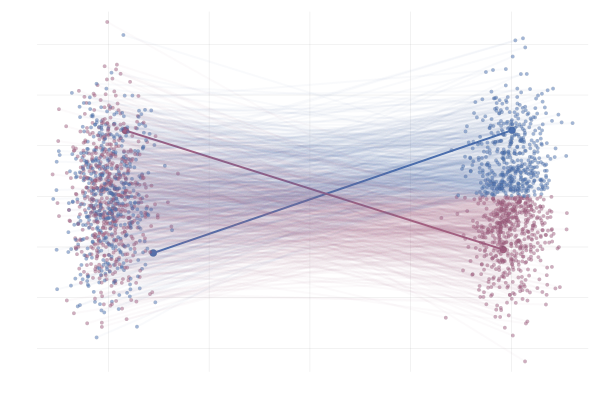
\includegraphics[width=\linewidth]{figs/g2g-vector-field-samples-cond}
			\end{figure}
		\end{minipage}%
		\begin{minipage}[t]{0.5\columnwidth}
			\begin{figure}
				\centering
				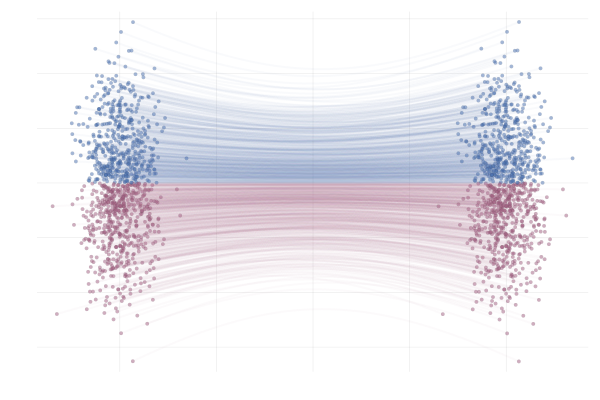
\includegraphics[width=\linewidth]{figs/g2g-forward_samples}
			\end{figure}
	\end{minipage}
	\myfootnotewithlink{https://mlg.eng.cam.ac.uk/blog/2024/01/20/flow-matching.html}{image credit: https://mlg.eng.cam.ac.uk/blog/2024/01/20/flow-matching.html}
\end{frame}
%=======
\subsection{Link with score-based models}
%=======
\begin{frame}{Score-based generative models through SDEs}
	\vspace{-0.3cm}
	\begin{block}{Training}
		\vspace{-0.7cm}
		\[
			\bbE_{\pi(\bx(0))} \bbE_{t \sim U[0, 1]} \bbE_{q(\bx(t) | \bx(0))}\bigl\| \bs_{\btheta}(\bx(t), t) - {\color{teal}\nabla_{\bx(t)} \log q(\bx(t) | \bx(0))} \bigr\|^2_2 
		\]
		\vspace{-0.5cm}
	\end{block}
	\begin{block}{Variance Exploding SDE (NCSN)}
		\vspace{-0.3cm}
		\[
			q(\bx(t) | \bx(0)) = \cN\left(\bx(0), \left[\sigma^2(t) - \sigma^2(0)\right] \cdot \bI\right), \quad \sigma(0) =0.
		\]
		\vspace{-0.5cm}
	\end{block}
	\begin{block}{Variance Preserving SDE (DDPM)}
		\vspace{-0.5cm}
		\[
			q(\bx(t) | \bx(0)) = \cN\left(\bx(0) \alpha(t), \left(1 - \alpha(t)^2\right) \cdot \bI\right); \quad \alpha(t) = e^{-\frac{1}{2} \int_0^t \beta(s) ds}
		\]
		\vspace{-0.5cm}
	\end{block}
	Flow matching uses the reverse time direction.
	\[
		\textbf{NCSN: } p(\bx | \bx_1) = \cN\left(\bx_1, \sigma^2_{1-t} \cdot \bI\right)
	\]
	\vspace{-0.5cm}
	\[
		\textbf{DDPM: } p(\bx | \bx_1) = \cN\left(\alpha_{1-t} \bx_1, \left(1 - \alpha_{1-t}^2\right) \cdot \bI\right)
	\]
	\vspace{-0.5cm}
	\myfootnotewithlink{https://arxiv.org/abs/2210.02747}{Lipman Y., et al. Flow Matching for Generative Modeling, 2022}
\end{frame}
%=======
\begin{frame}{Flow matching vs score-based SDE models}
	\begin{block}{Flow matching probability path}
		\vspace{-0.3cm}
		\[
			p_t(\bx | \bx_1) = \cN\left(t \bx_1, (1-t)^2 \bI\right); \quad \bff(\bx, \bx_1, t) = \frac{\bx_1  - \bx}{1-t}
		\]
		\vspace{-0.3cm}
		\[
	 		\frac{d\bx}{dt} = \bff(\bx, \bx_1, t) =  \bmu_t'(\bx_1) + \frac{\bsigma_t'(\bx_1)}{\bsigma_t(\bx_1)} \odot (\bx - \bmu_t(\bx_1))
		\]
	\end{block}
	\begin{block}{Variance Exploding SDE probability path}
		\vspace{-0.3cm}
		\[
				p_t(\bx | \bx_1) = \cN\left(\bx_1, \sigma^2_{1-t}  \bI\right) \quad \Rightarrow \quad 
				\bff(\bx, \bx_1, t) = - \frac{\sigma'_{1-t}}{\sigma_{1-t}} \cdot (\bx - \bx_1)
		\]
		\vspace{-0.3cm}
	\end{block}
	\begin{block}{Variance Preserving SDE probability path}
		\vspace{-0.3cm}
		{\small
		\[
			p_t(\bx | \bx_1) = \cN\left(\alpha_{1-t}  \bx_1, (1 - \alpha^2_{1-t})  \bI \right)  \, \Rightarrow \, 
		\bff(\bx, \bx_1, t) = \frac{\alpha'_{1-t}}{1 - \alpha^2_{1-t}}\cdot \left(\alpha_{1-t}  \bx - \bx_1\right)
		\]
		}
	\end{block}
	\myfootnotewithlink{https://arxiv.org/abs/2210.02747}{Lipman Y., et al. Flow Matching for Generative Modeling, 2022}
\end{frame}
%=======
\begin{frame}{Flow matching vs score-based SDE models}
	\begin{block}{SDE vector field}
		\vspace{-0.3cm}
		\[
			\bff(\bx, \bx_1, t) = \frac{\alpha'_{1-t}}{1 - \alpha^2_{1-t}}\cdot \left(\alpha_{1-t}  \bx - \bx_1\right)
		\]
		\vspace{-0.5cm}
		\begin{figure}
			\raggedleft
			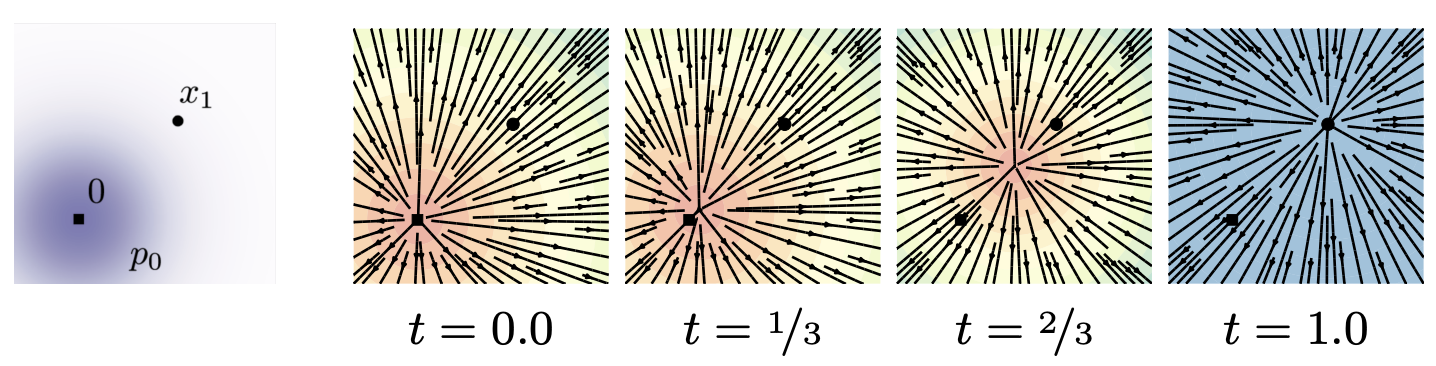
\includegraphics[width=0.8\linewidth]{figs/diff_cond_path}
		\end{figure}
		\vspace{-0.5cm}
	\end{block}
	\begin{block}{FM vector field}
		\vspace{-0.5cm}
		\[
			\bff(\bx, \bx_1, t) = - \frac{\sigma'_{1-t}}{\sigma_{1-t}} \cdot (\bx - \bx_1)
		\]
		\vspace{-0.5cm}
		\begin{figure}
			\raggedleft
			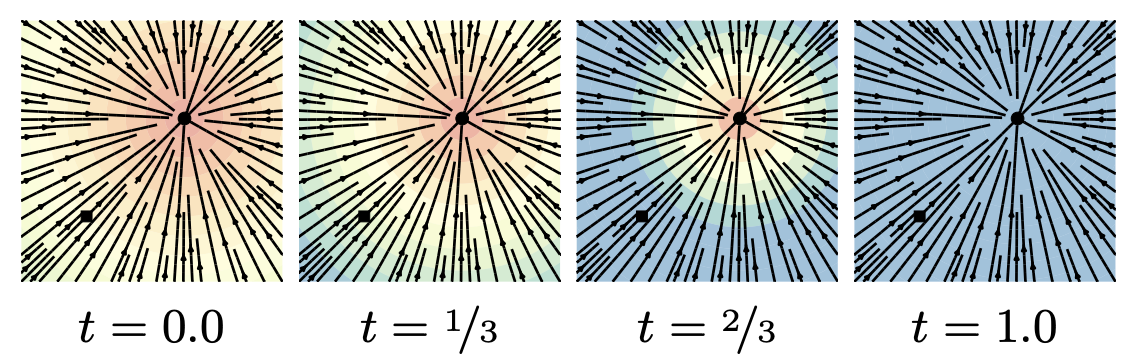
\includegraphics[width=0.6\linewidth]{figs/ot_cond_path}
		\end{figure}
	\end{block}
	\myfootnotewithlink{https://arxiv.org/abs/2210.02747}{Lipman Y., et al. Flow Matching for Generative Modeling, 2022}
\end{frame}
%=======
\begin{frame}{Flow matching vs score-based SDE models}
	\begin{block}{Trajectories}
		\vspace{-0.3cm}
		\begin{figure}
			\centering
			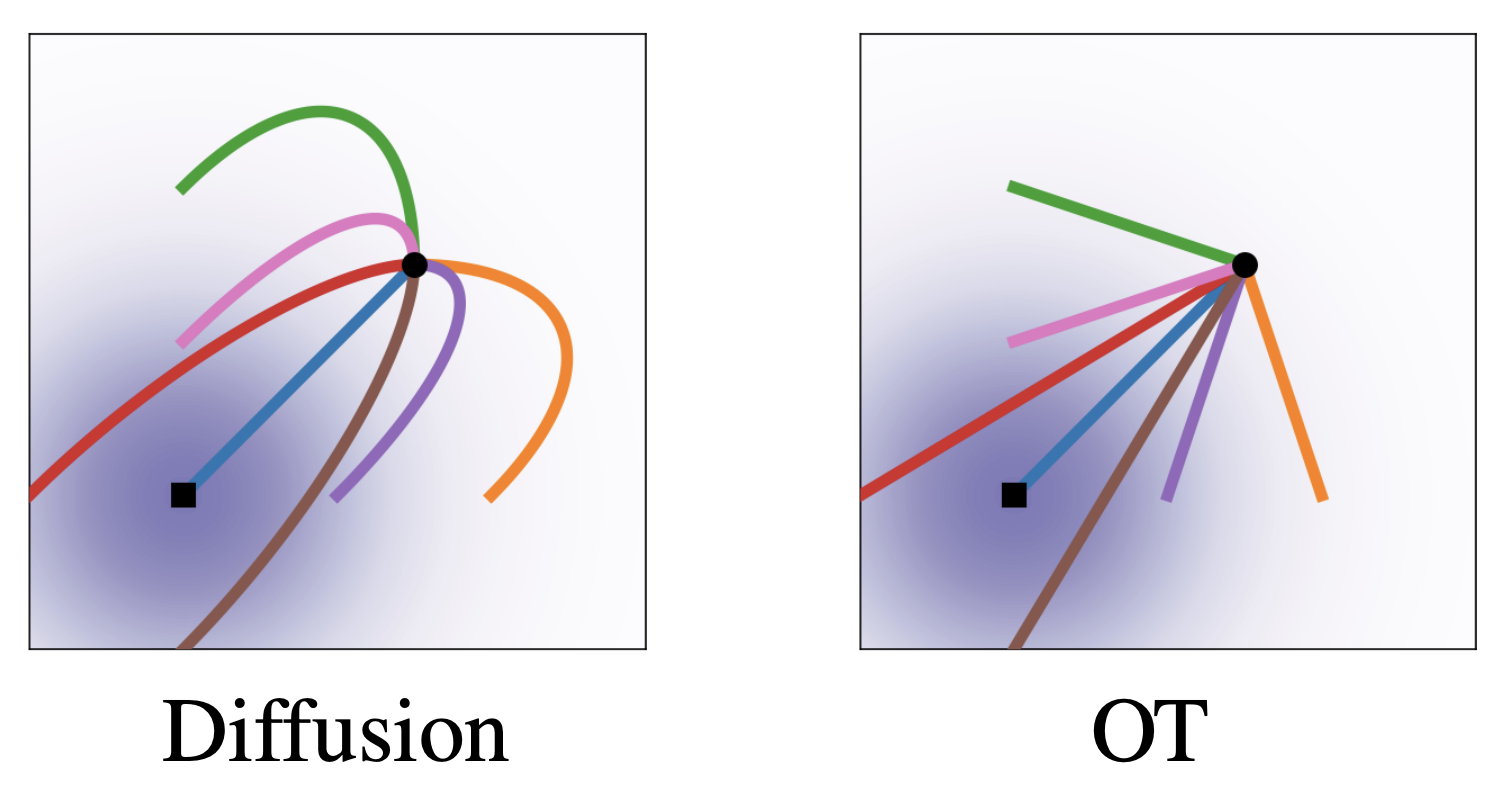
\includegraphics[width=0.6\linewidth]{figs/trajectories}
		\end{figure}
		\vspace{-0.3cm}
	\end{block}
	\begin{figure}
		\centering
		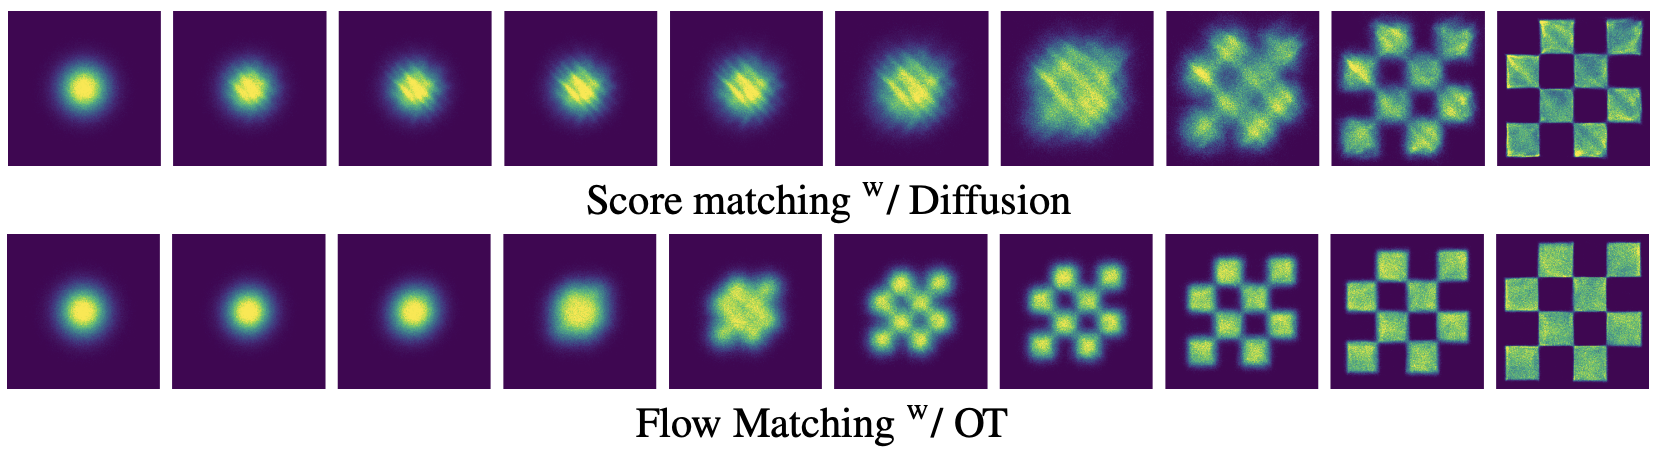
\includegraphics[width=\linewidth]{figs/2d-generation}
	\end{figure}
	\myfootnotewithlink{https://arxiv.org/abs/2210.02747}{Lipman Y., et al. Flow Matching for Generative Modeling, 2022}
\end{frame}
%=======
\subsection{Linear interpolation}
%=======
\begin{frame}{Pair conditioning}
	\begin{block}{Conditional Flow Matching}
		\vspace{-0.3cm}
		\[
			\bbE_{t \sim U[0, 1]} \bbE_{\bz \sim p(\bz)} \bbE_{\bx \sim p_t(\bx | \bz)}\left\| \bff(\bx, \bz, t) - \bff_{\btheta}(\bx, t) \right\|^2 \rightarrow \min_{\btheta}
		\]
		\vspace{-0.3cm}
	\end{block}
	\begin{block}{Conditioning latent variable}
		Let choose $\bz = (\bx_0, \bx_1)$. Then $p(\bz) = p_0(\bx_0) p_1(\bx_1)$.
		\[
			p_t(\bx) = \int p_t(\bx | \bx_0, \bx_1) p_0(\bx_0) p_1(\bx_1) d \bx_0 d \bx_1
		\]
	\end{block}
	We need to ensure boundary constraints:
	\[
		\begin{cases}
			p(\bx) = \bbE_{p(\bz)} p_0(\bx | \bz); {\color{gray}(= \cN(0, \bI))} \\
			\pi(\bx) = \bbE_{p(\bz)} p_1(\bx | \bz).
		\end{cases}
		\, \Rightarrow \, 
		\begin{cases}
			p_0(\bx | \bx_0, \bx_1) = \delta(\bx - \bx_0); \\
			p_1(\bx | \bx_0, \bx_1) = \delta(\bx - \bx_1).
		\end{cases}
	\]
	\vspace{-0.3cm}
	\myfootnotewithlink{https://arxiv.org/abs/2210.02747}{Lipman Y., et al. Flow Matching for Generative Modeling, 2022}
\end{frame}
%=======
\begin{frame}{Linear interpolation}
	\[
		p_0(\bx | \bx_0, \bx_1) = \delta(\bx - \bx_0); \quad p_1(\bx | \bx_0, \bx_1) = \delta(\bx - \bx_1).
	\]
	
	\begin{block}{Gaussian conditional probability path}
		\vspace{-0.5cm}
		{\small
		\[
			p_t(\bx | \bx_0, \bx_1) = \cN\left(\bmu_t(\bx_0, \bx_1), \bsigma_t^2(\bx_0, \bx_1)\right); \quad \bx_t = \bmu_t(\bx_0, \bx_1) +  \bsigma_t^2(\bx_0, \bx_1) \odot \bx_0.
		\]
		}
		\vspace{-0.6cm}
	\end{block}
	Let consider straight conditional paths	
	\[
		\begin{cases}
			\bmu_t(\bx_1) = t \bx_1 + (1 - t) \bx_0; \\
			\bsigma_t(\bx_1) = 0.
		\end{cases}
		\quad \Rightarrow \quad 
		\begin{cases}
			p_0(\bx | \bx_0, \bx_1) = \delta(\bx - \bx_0); \\
			p_1(\bx | \bx_0, \bx_1) = \delta(\bx - \bx_1).
		\end{cases}
	\]
	\vspace{-0.3cm}
	\begin{figure}
		\centering
		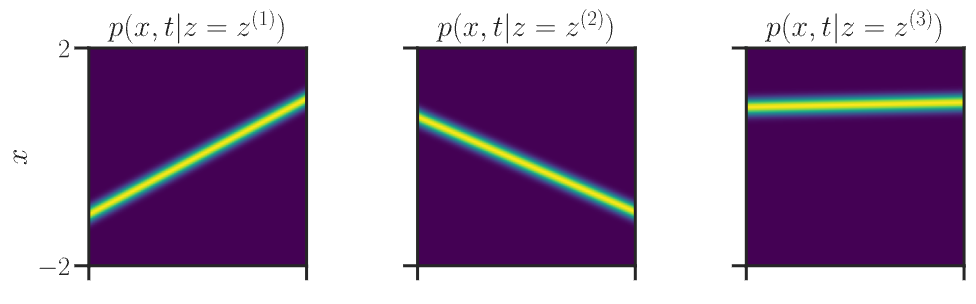
\includegraphics[width=\linewidth]{figs/linear_paths}
	\end{figure}
	\myfootnotewithlink{https://dl.heeere.com/conditional-flow-matching/blog/conditional-flow-matching}{image credit: A Visual Dive into Conditional Flow Matching}
\end{frame}
%=======
\begin{frame}{Flow Matching}
	Let consider straight conditional paths	
	\[
		\begin{cases}
			\bmu_t(\bx_0, \bx_1) = t \bx_1 + (1 - t) \bx_0; \\
			\bsigma_t(\bx_0, \bx_1) = 0.
		\end{cases}
		\, \Rightarrow \, 
		\begin{cases}
			p_t(\bx | \bx_0, \bx_1) = \cN\left(t \bx_1 + (1-t) \bx_0, 0\right); \\
		 	\bx_t = t \bx_1 + (1 - t) \bx_0. \\
		 \end{cases}
	\]
	\[
		 \frac{d\bx}{dt} = \bx_1 - \bx_0.
	\]
	\myfootnotewithlink{https://arxiv.org/abs/2210.02747}{Lipman Y., et al. Flow Matching for Generative Modeling, 2022}
\end{frame}
%=======
\begin{frame}{Flow Matching}
	\begin{figure}
		\centering
		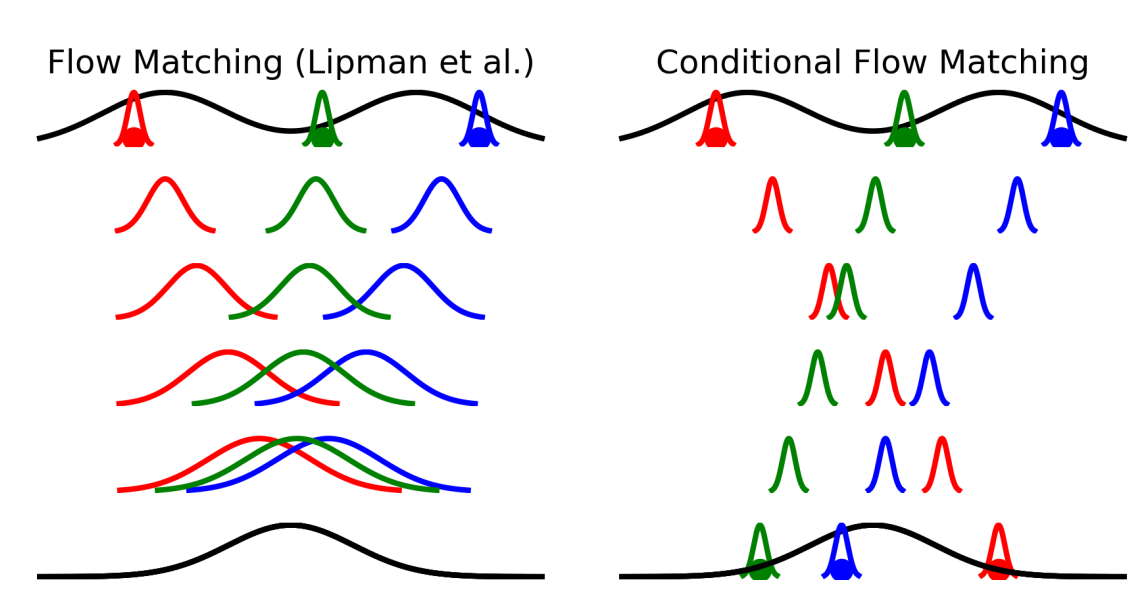
\includegraphics[width=\linewidth]{figs/compare_conditionings}
	\end{figure}
	\myfootnotewithlink{https://arxiv.org/pdf/2302.00482}{Tong A., et al. Improving and Generalizing Flow-Based Generative Models with Minibatch Optimal Transport, 2023}
\end{frame}
%=======
\subsection{Rectified flows}
%=======
\begin{frame}{Rectified flows}
	\begin{figure}
		\centering
		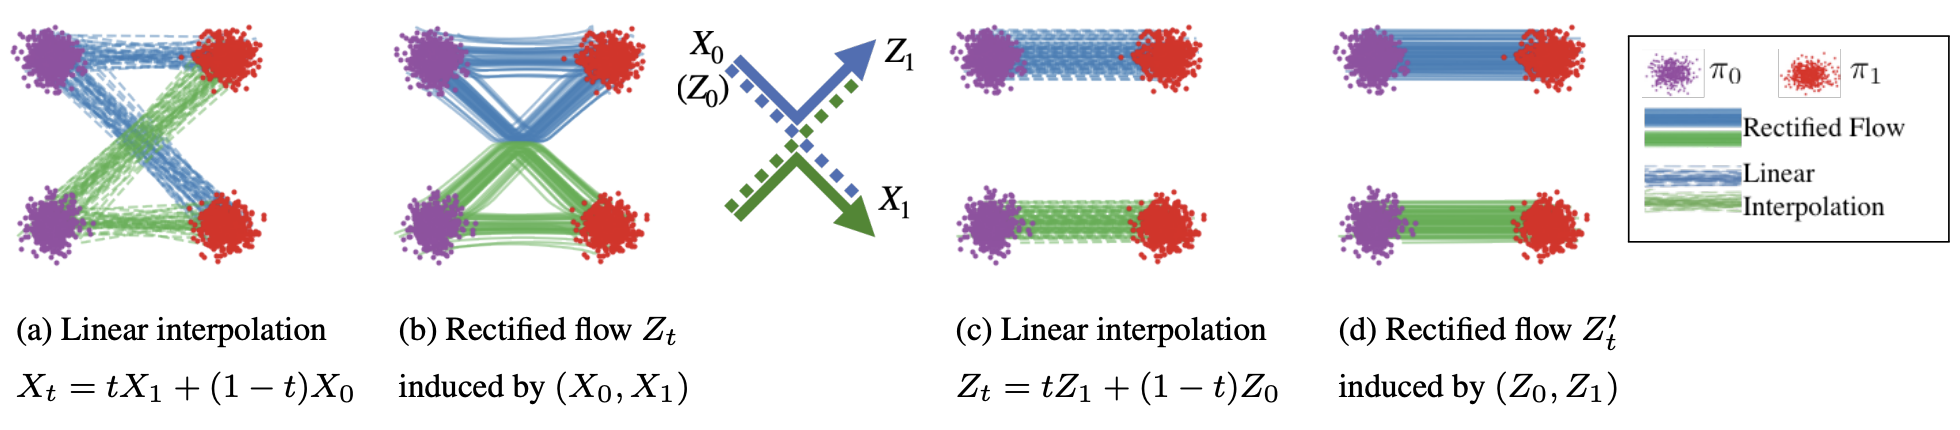
\includegraphics[width=\linewidth]{figs/rectified_flow}
	\end{figure}
	\begin{figure}
		\centering
		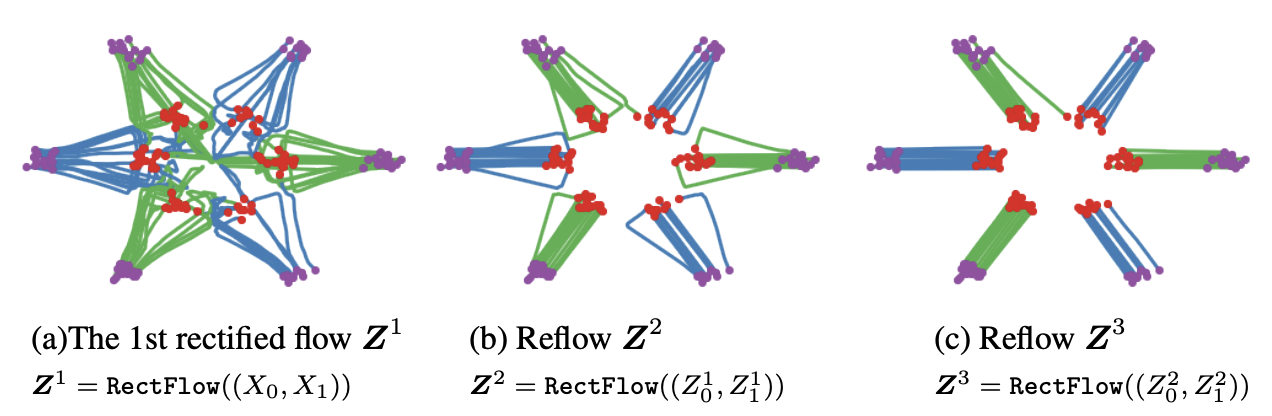
\includegraphics[width=\linewidth]{figs/star_fig}
	\end{figure}
	\myfootnotewithlink{https://arxiv.org/abs/2209.03003}{Liu X., et al. Flow Straight and Fast: Learning to Generate and Transfer Data with Rectified Flow, 2022}
\end{frame}
%=======
\begin{frame}{Rectified flows}
	\begin{figure}
		\centering
		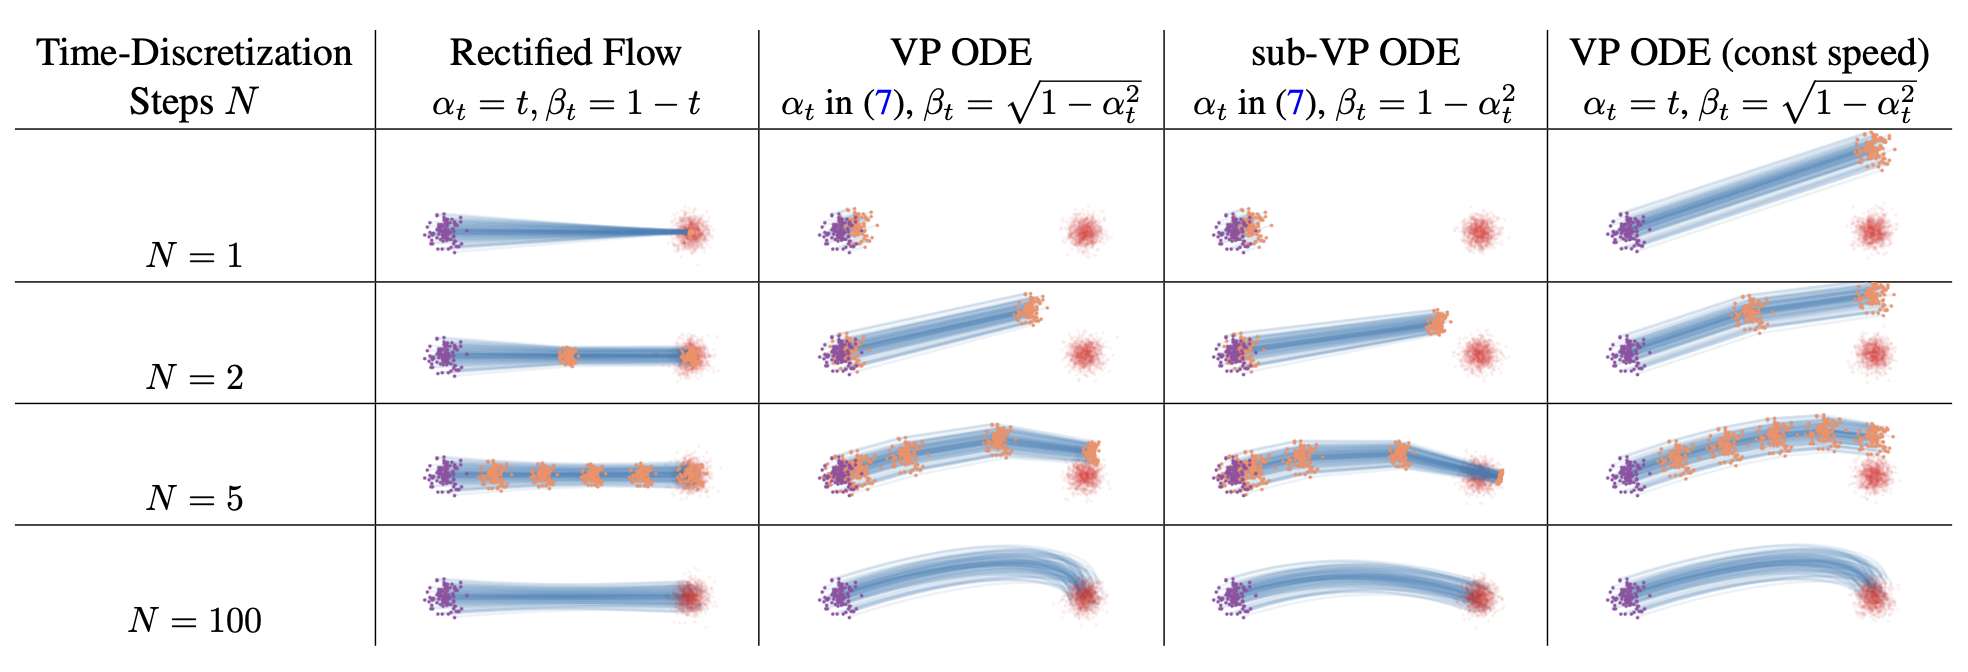
\includegraphics[width=\linewidth]{figs/combined_vp}
	\end{figure}
	\myfootnotewithlink{https://arxiv.org/abs/2209.03003}{Liu X., et al. Flow Straight and Fast: Learning to Generate and Transfer Data with Rectified Flow, 2022}
\end{frame}
%=======
\begin{frame}{Rectified flows: Stable Diffusion 3}
	\begin{figure}
		\centering
		\includegraphics[width=\linewidth]{figs/sd3}
	\end{figure}
	\myfootnotewithlink{https://arxiv.org/pdf/2403.03206}{Esser P., et al. Scaling Rectified Flow Transformers for High-Resolution Image Synthesis, 2024}
\end{frame}
%=======
\section{Latent space models}
%=======
\subsection{Score-based models}
%=======
\begin{frame}{Latent space models}
	\begin{block}{Score-based models (diffusion)}
		\vspace{-0.3cm}
		\begin{figure}
			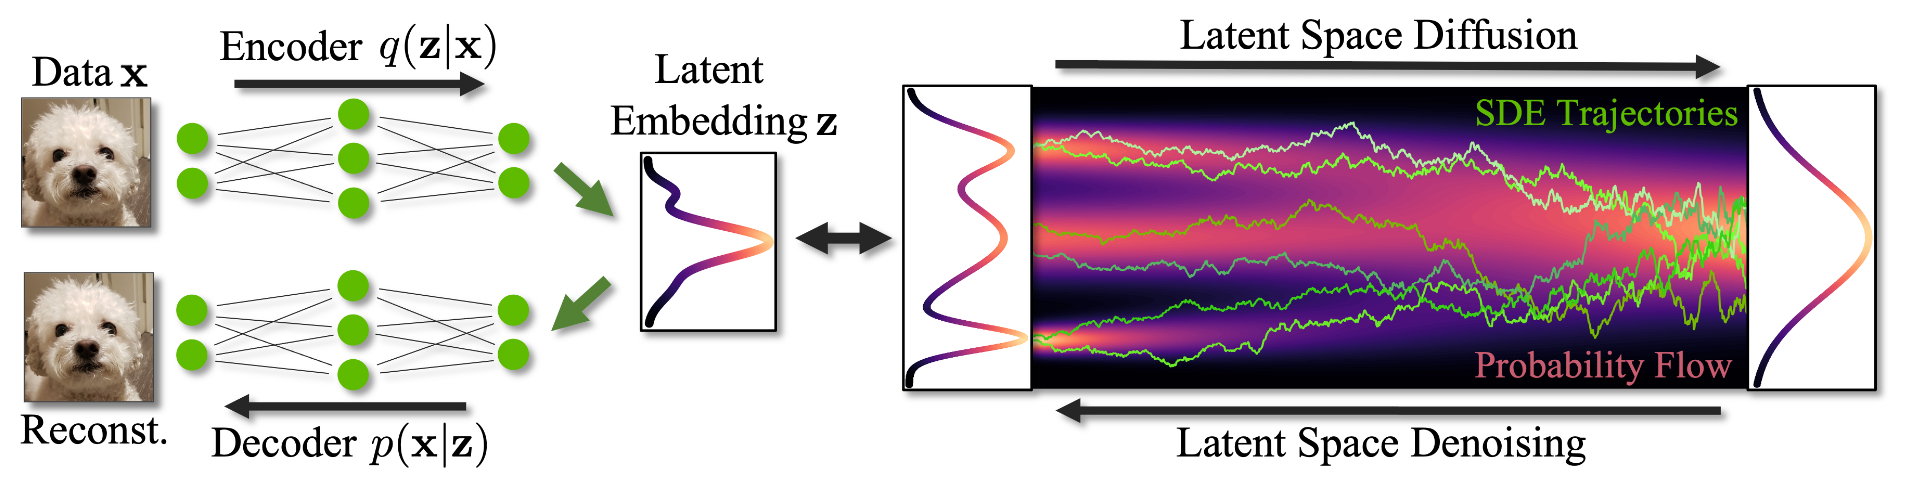
\includegraphics[width=\linewidth]{figs/latent_diffusion}
		\end{figure}
		\vspace{-0.3cm}
	\end{block}
	\begin{block}{Flow matching}
		\vspace{-0.3cm}
		\begin{figure}
			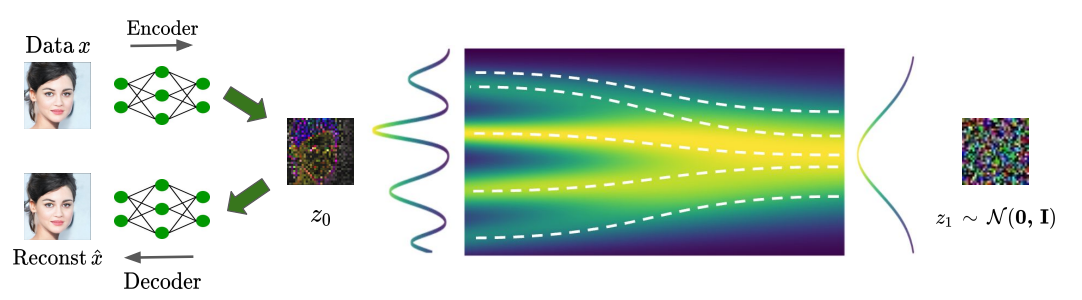
\includegraphics[width=\linewidth]{figs/latent_flow_matching}
		\end{figure}
	\end{block}

	\myfootnote{\href{https://arxiv.org/abs/2307.08698}{Dao Q. et al. Flow Matching in Latent Space, 2023} \\ \href{https://neurips2023-ldm-tutorial.github.io/}{NeurIPS 2023 Tutorial: Latent Diffusion Models: Is the Generative AI Revolution Happening in Latent Space?}}
\end{frame}
%=======
\subsection{Autoregressive models}
%=======
\begin{frame}{Vector Quantized VAE (VQ-VAE) }
	\begin{block}{Vector quantization}
		Define the dictionary space $\{\be_k\}_{k=1}^K$, where $\be_k \in \bbR^C$, $K$ is the size of the dictionary.
		\vspace{-0.5cm}
		\begin{minipage}[t]{0.45\columnwidth}
			\[
				\bz_q = \bq (\bz) = \be_{k^*}
			\] 
			Here $k^* = \argmin_k \| \bz - \be_k \|$.
		\end{minipage}%
		\begin{minipage}[t]{0.55\columnwidth}
			\vspace{-0.5cm}
			\begin{figure}
				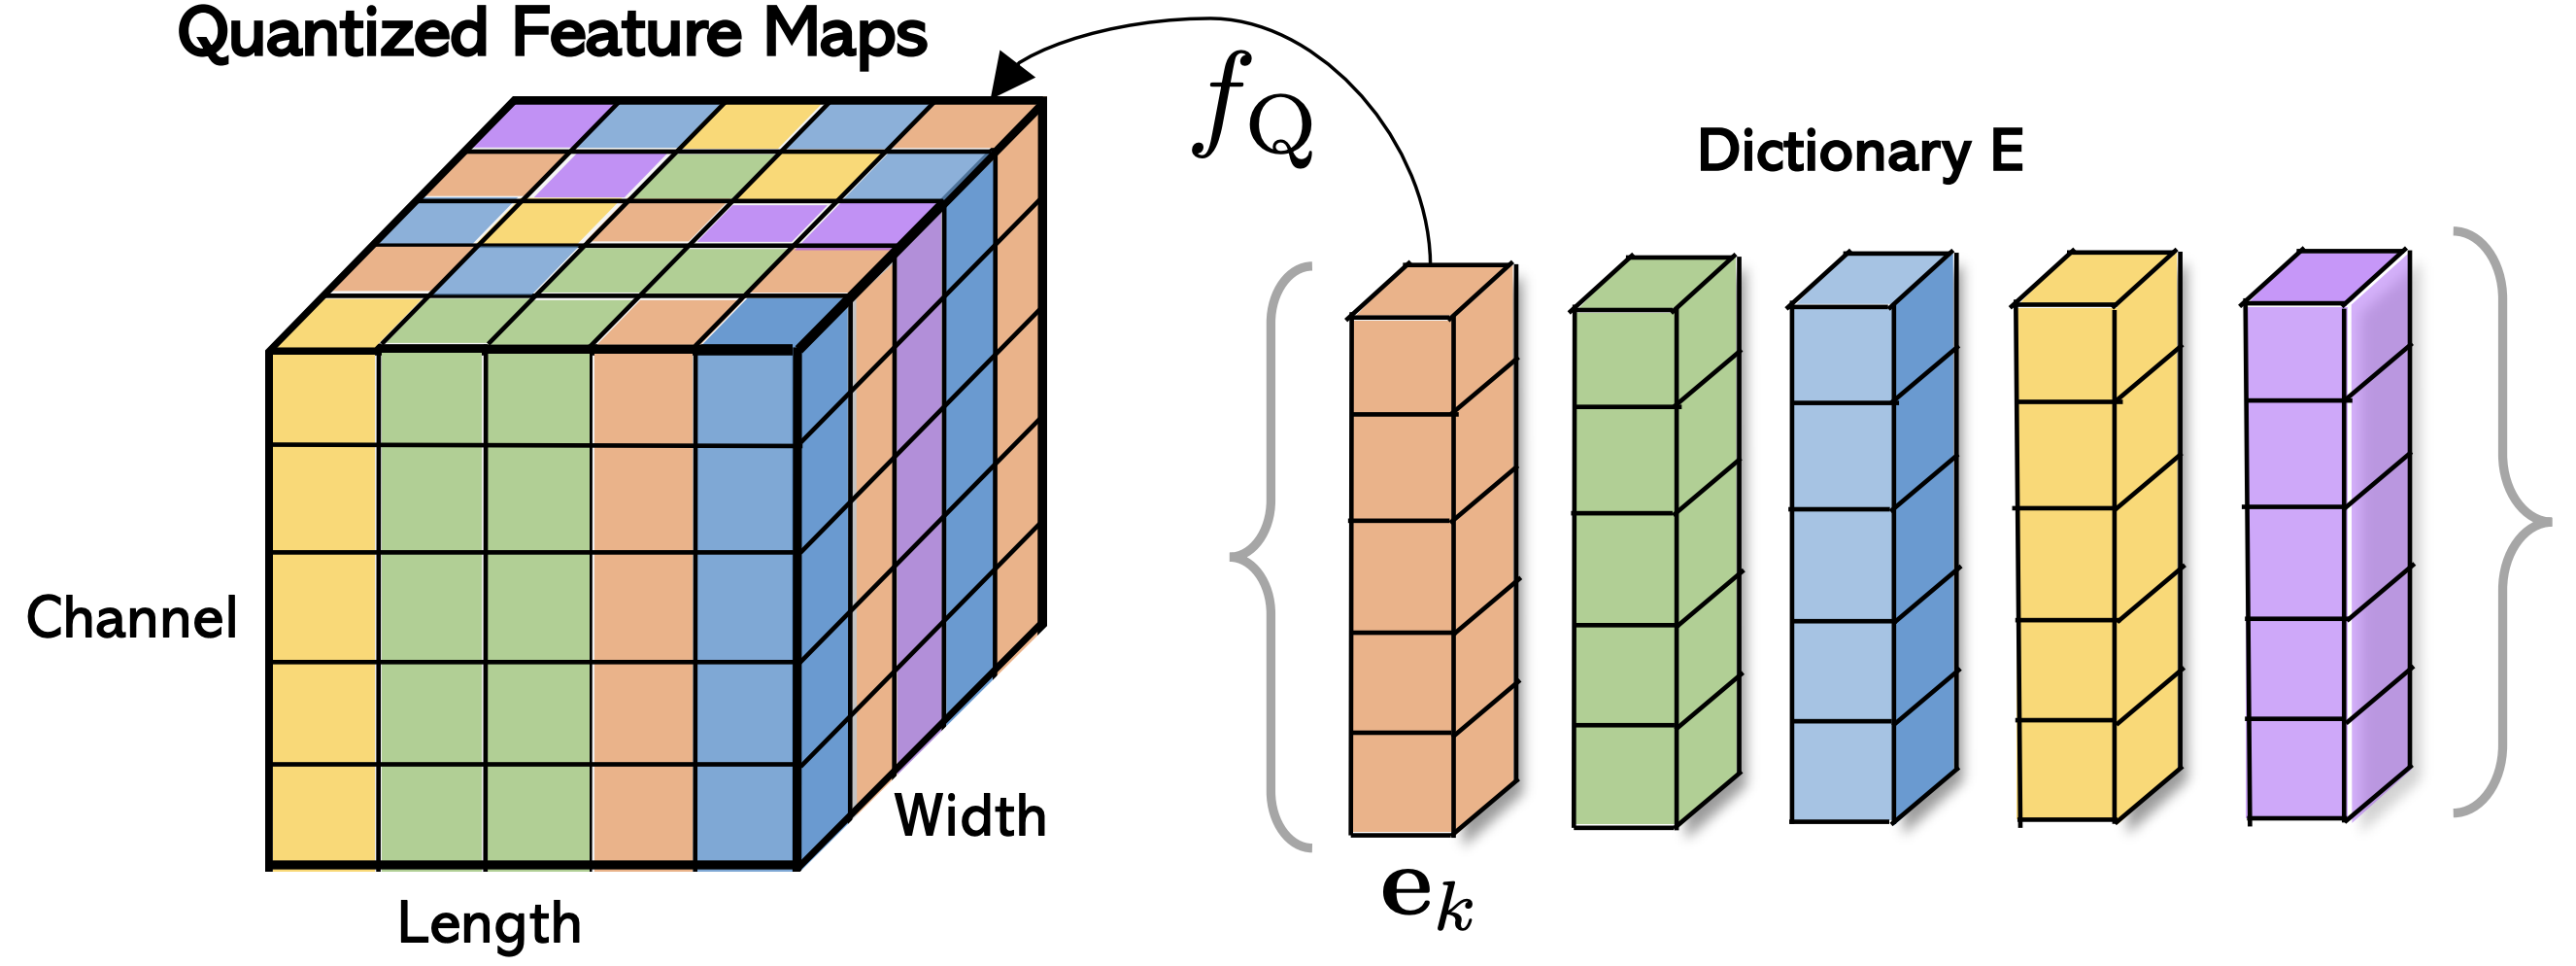
\includegraphics[width=\linewidth]{figs/fqgan_cnn}
			\end{figure}
		\end{minipage}		
	\end{block}
	\[
		\cL_{\bphi, \btheta}(\bx)  =  \log p(\bx | \bz_q, \btheta) - \log K
	\]
	\vspace{-0.5cm}
	\begin{figure}
		\centering
		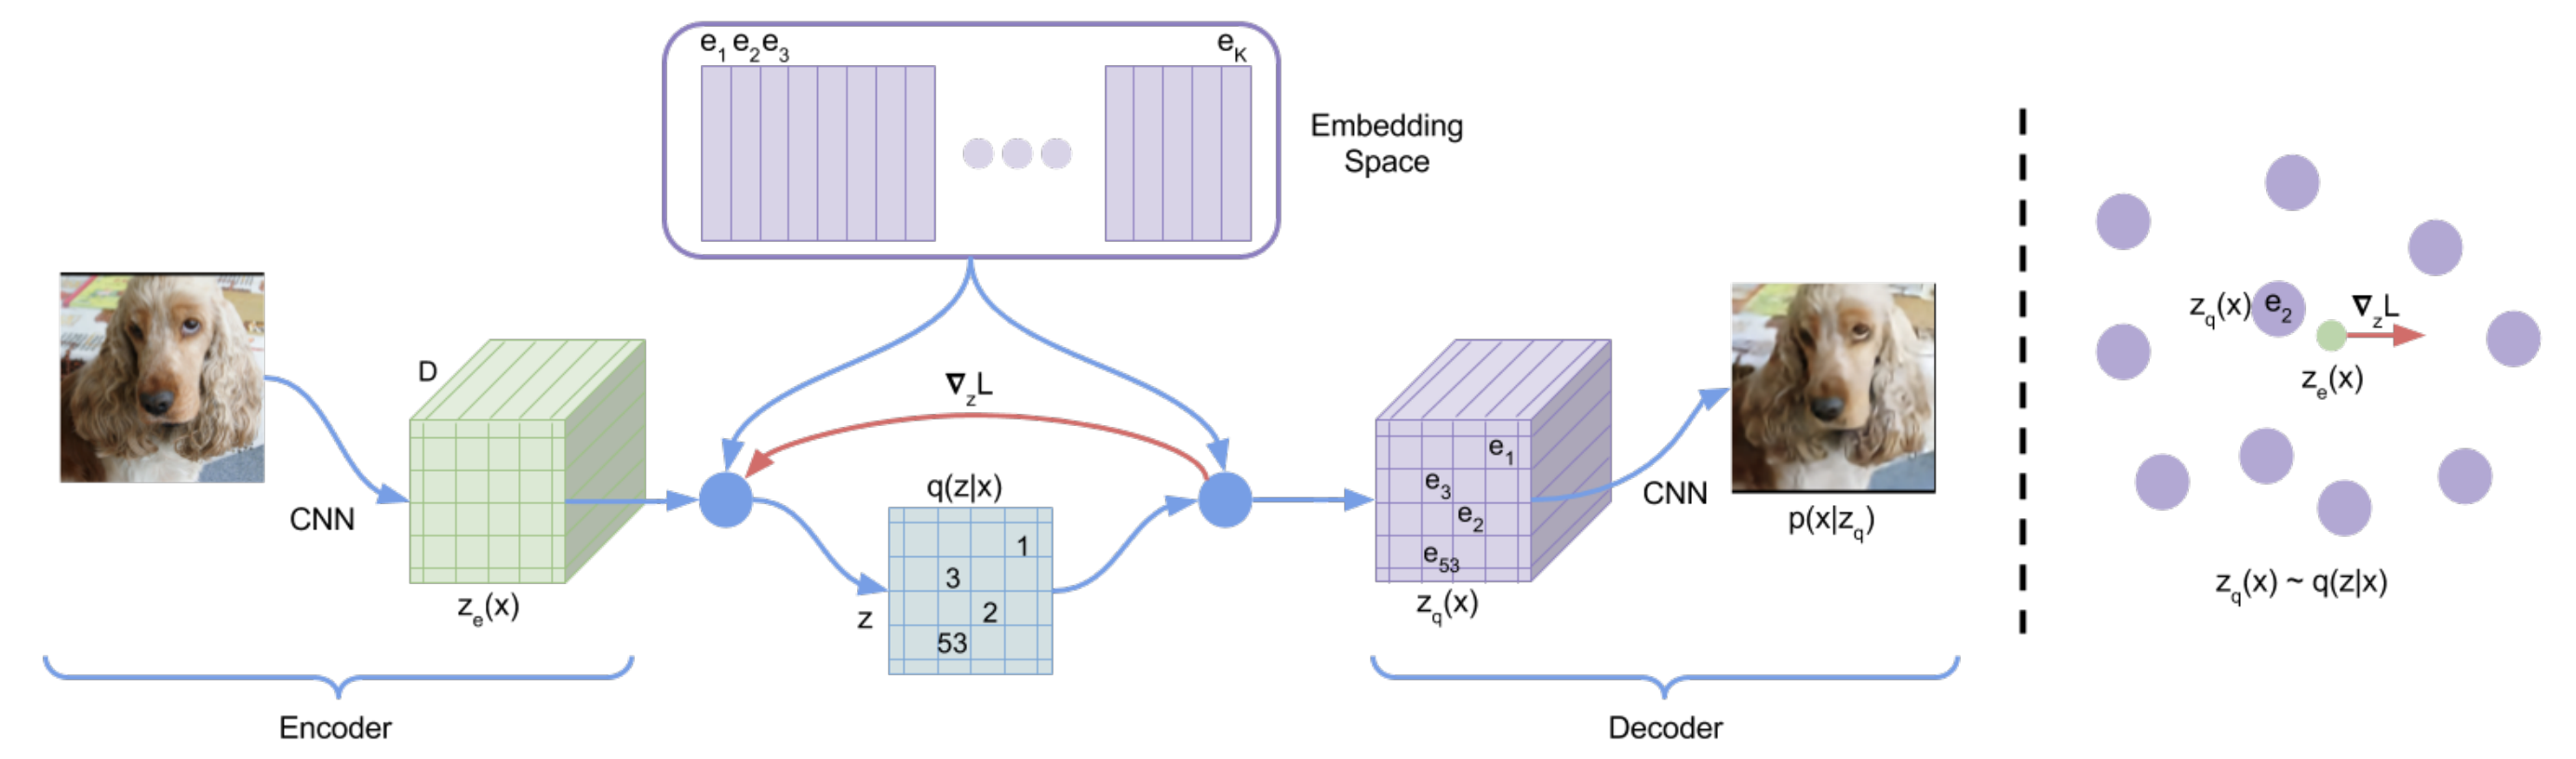
\includegraphics[width=\linewidth]{figs/vqvae}
	\end{figure}
	\myfootnote{\href{https://arxiv.org/abs/2004.02088}{Zhao Y. et al. Feature Quantization Improves GAN Training, 2020} \\ \href{https://arxiv.org/abs/1711.00937}{Oord A., Vinyals O., Kavukcuoglu K. Neural Discrete Representation Learning, 2017}}
\end{frame}
%=======
\begin{frame}{Vector Quantized GAN}
	\begin{itemize}
		\item Use VQVAE model and objective.
		\item Add adversarial loss between generated and real images to improve the visual quality of the reconstructions.
	\end{itemize}
	\begin{figure}
		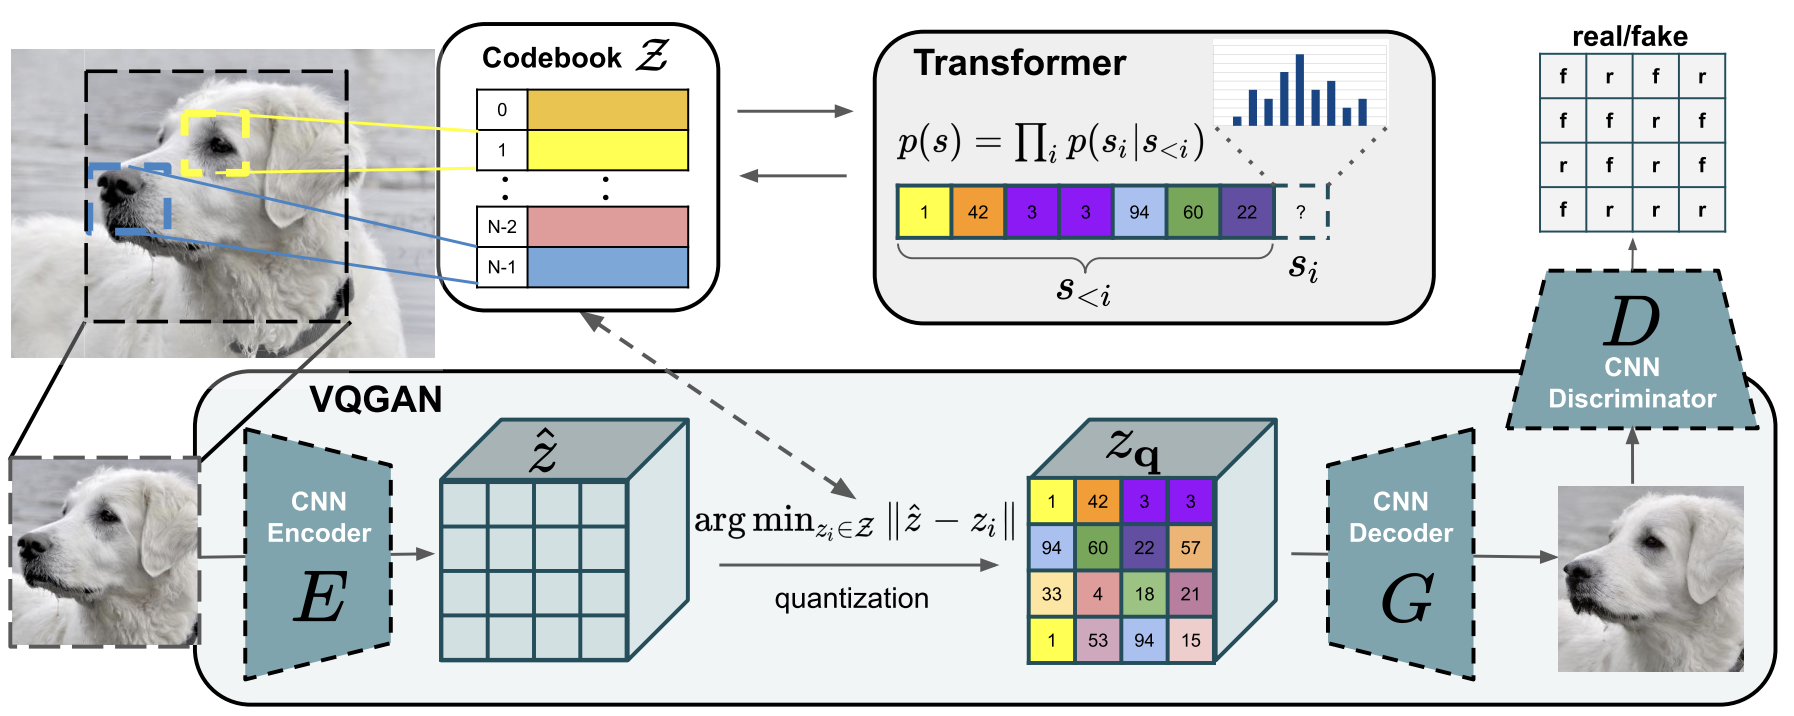
\includegraphics[width=\linewidth]{figs/vqgan}
	\end{figure}
	
	\myfootnotewithlink{https://arxiv.org/abs/2012.09841}{Esser P. et al. Taming Transformers for High-Resolution Image Synthesis, 2020}
\end{frame}
%=======
\begin{frame}{LlamaGen: pure autoregression}
	\begin{itemize}
		\item Use VQGAN encoder to map images to the discrete latent space of the codebook vectors.
		\item Learn the pure autoregression model (Llama-based) in the latent space.
		\item Use VQGAN decoder to map the discrete space tokens to the image space.
	\end{itemize}
	\begin{figure}
		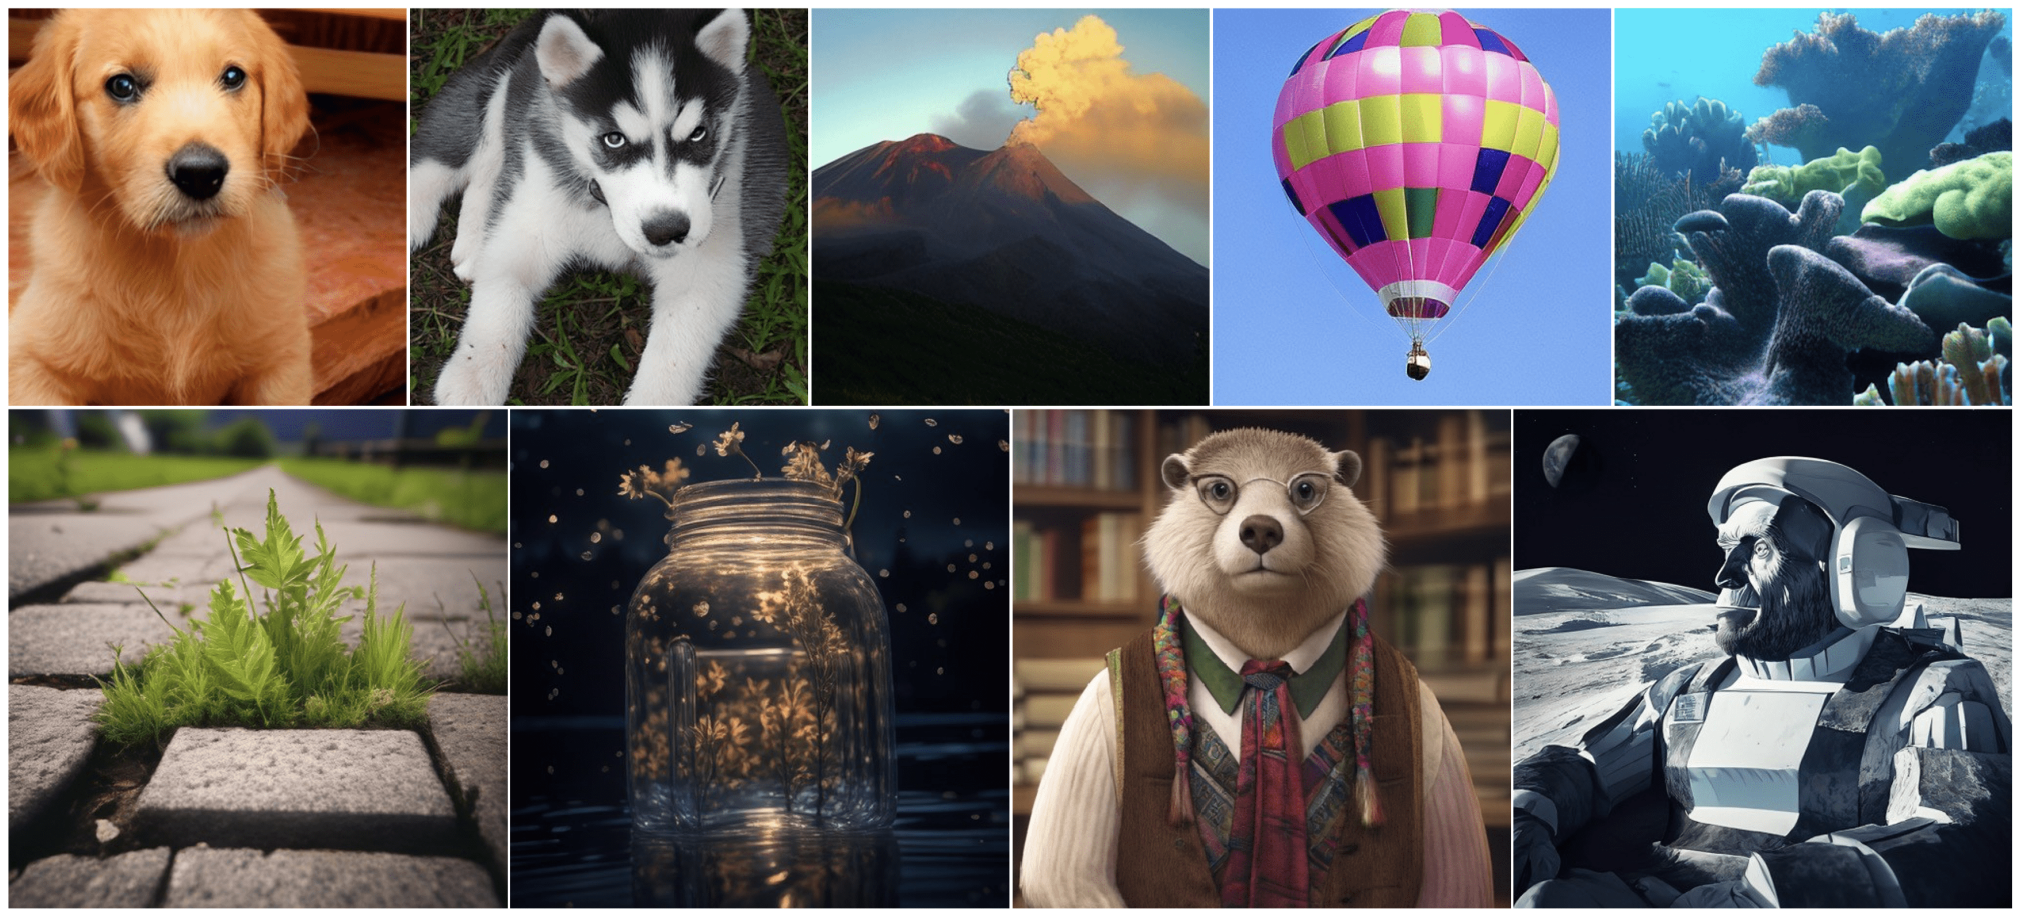
\includegraphics[width=0.9\linewidth]{figs/llamagen_samples}
	\end{figure}
	
	\myfootnotewithlink{https://arxiv.org/pdf/2406.06525}{Sun P. et al. Autoregressive Model Beats Diffusion: Llama for Scalable Image Generation, 2024}
\end{frame}
%=======
\begin{frame}{Visual Autoregressive Modeling (VAR)}
	\begin{figure}
		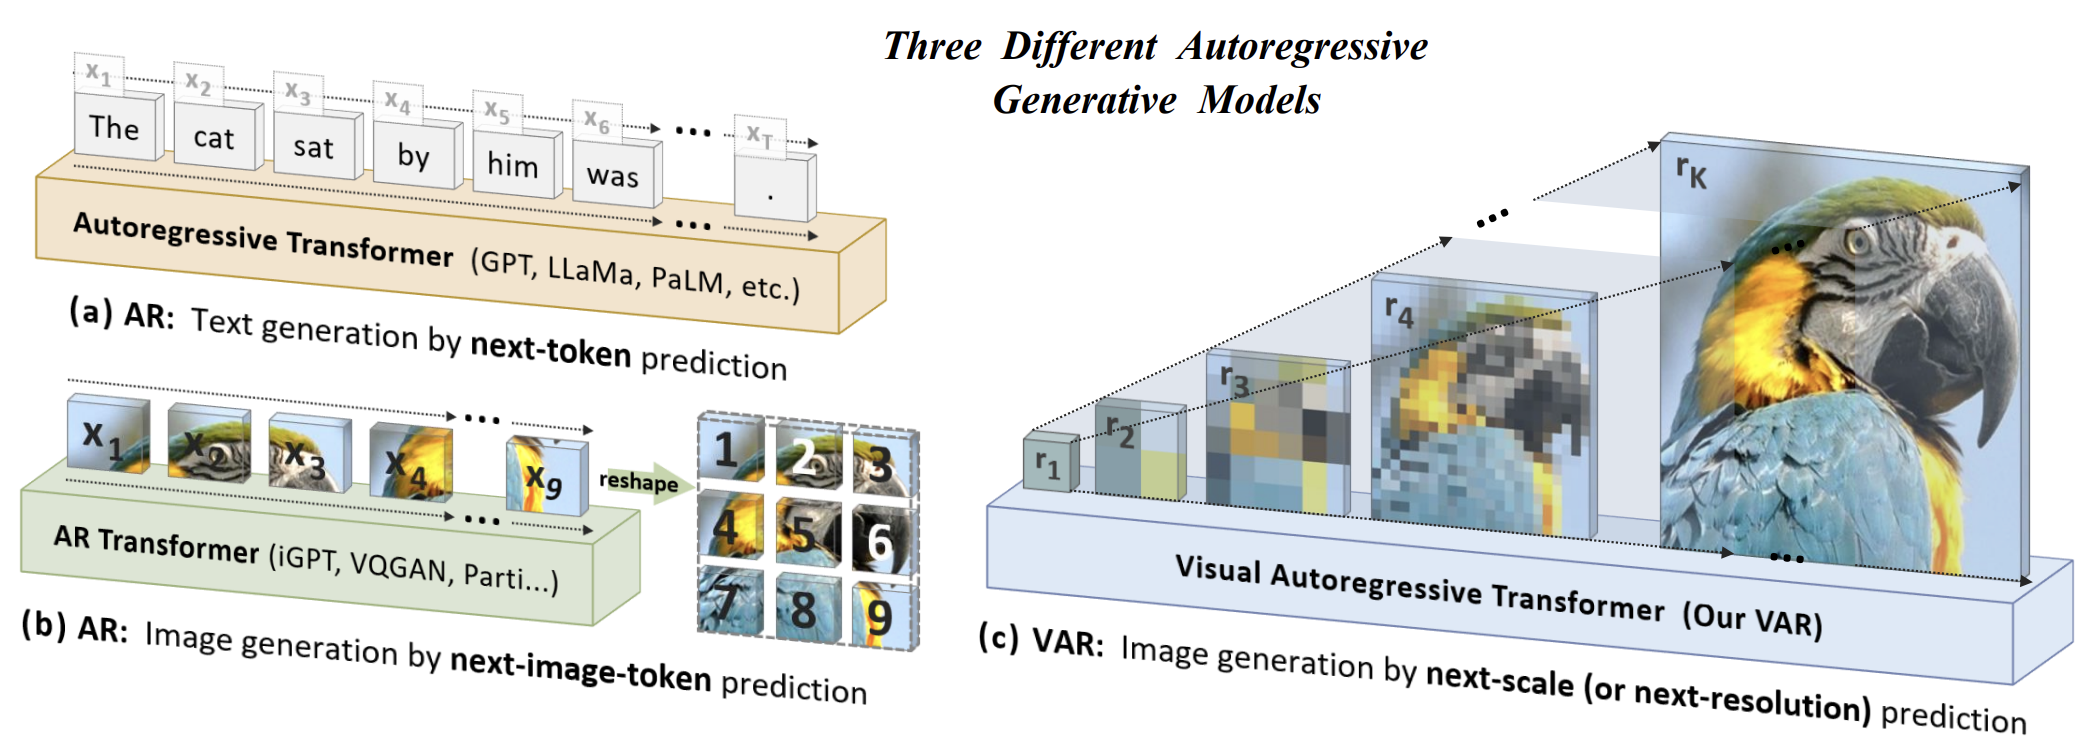
\includegraphics[width=\linewidth]{figs/var_idea}
	\end{figure}
	\begin{figure}
		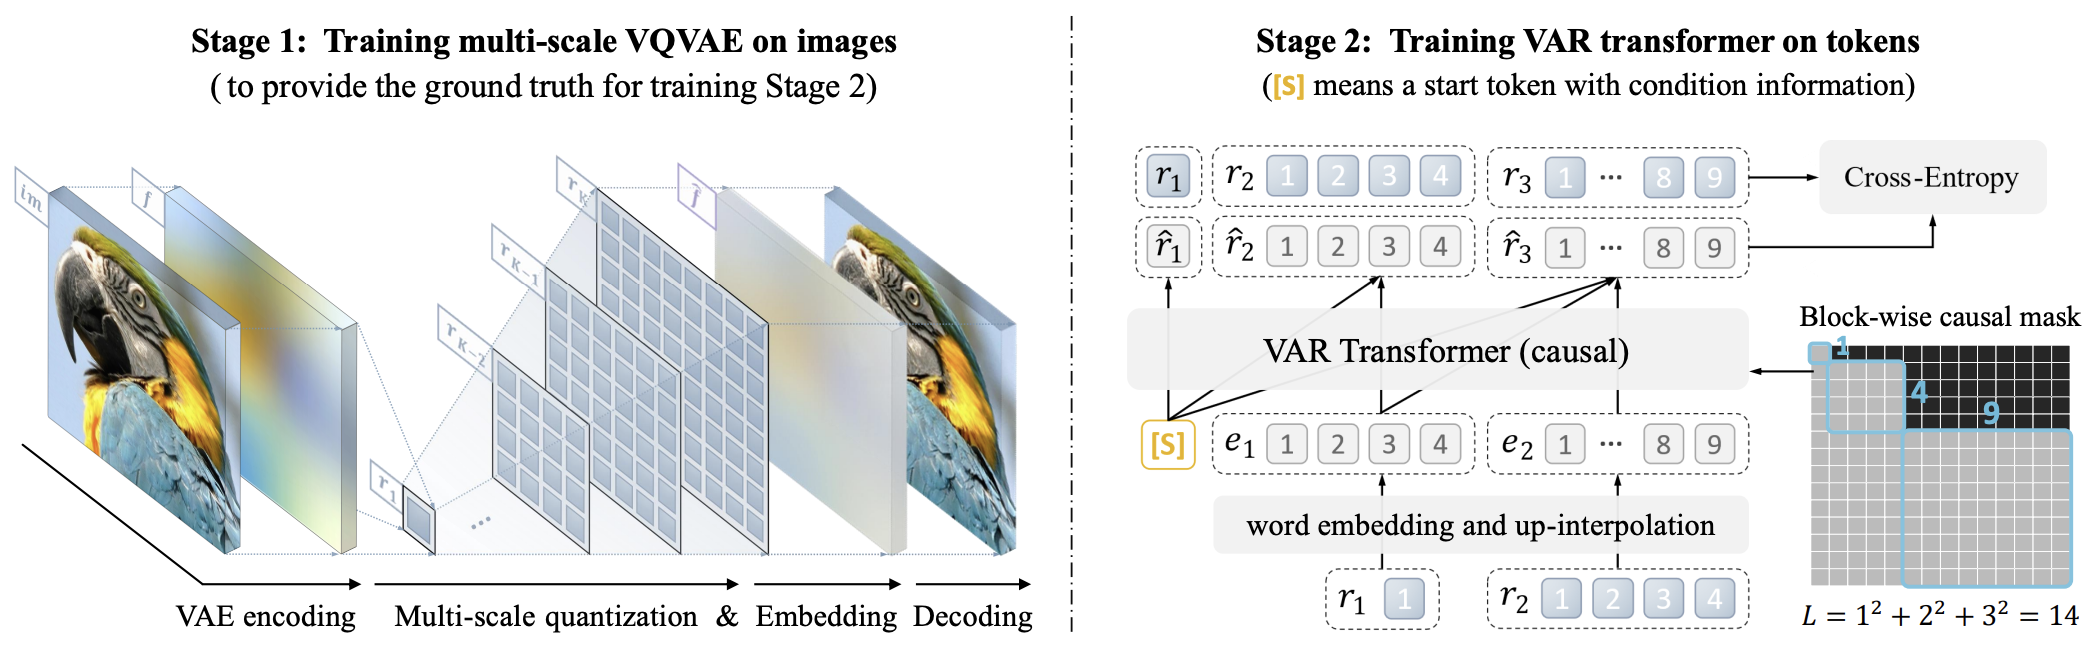
\includegraphics[width=\linewidth]{figs/var_training}
	\end{figure}
	\myfootnotewithlink{https://arxiv.org/pdf/2404.02905}{Tean K. et al. Visual Autoregressive Modeling: Scalable Image Generation via Next-Scale Prediction, 2024}
\end{frame}
%=======
\section{The worst course overview}
%=======
\begin{frame}{The worst course overview :)}
	\begin{figure}
		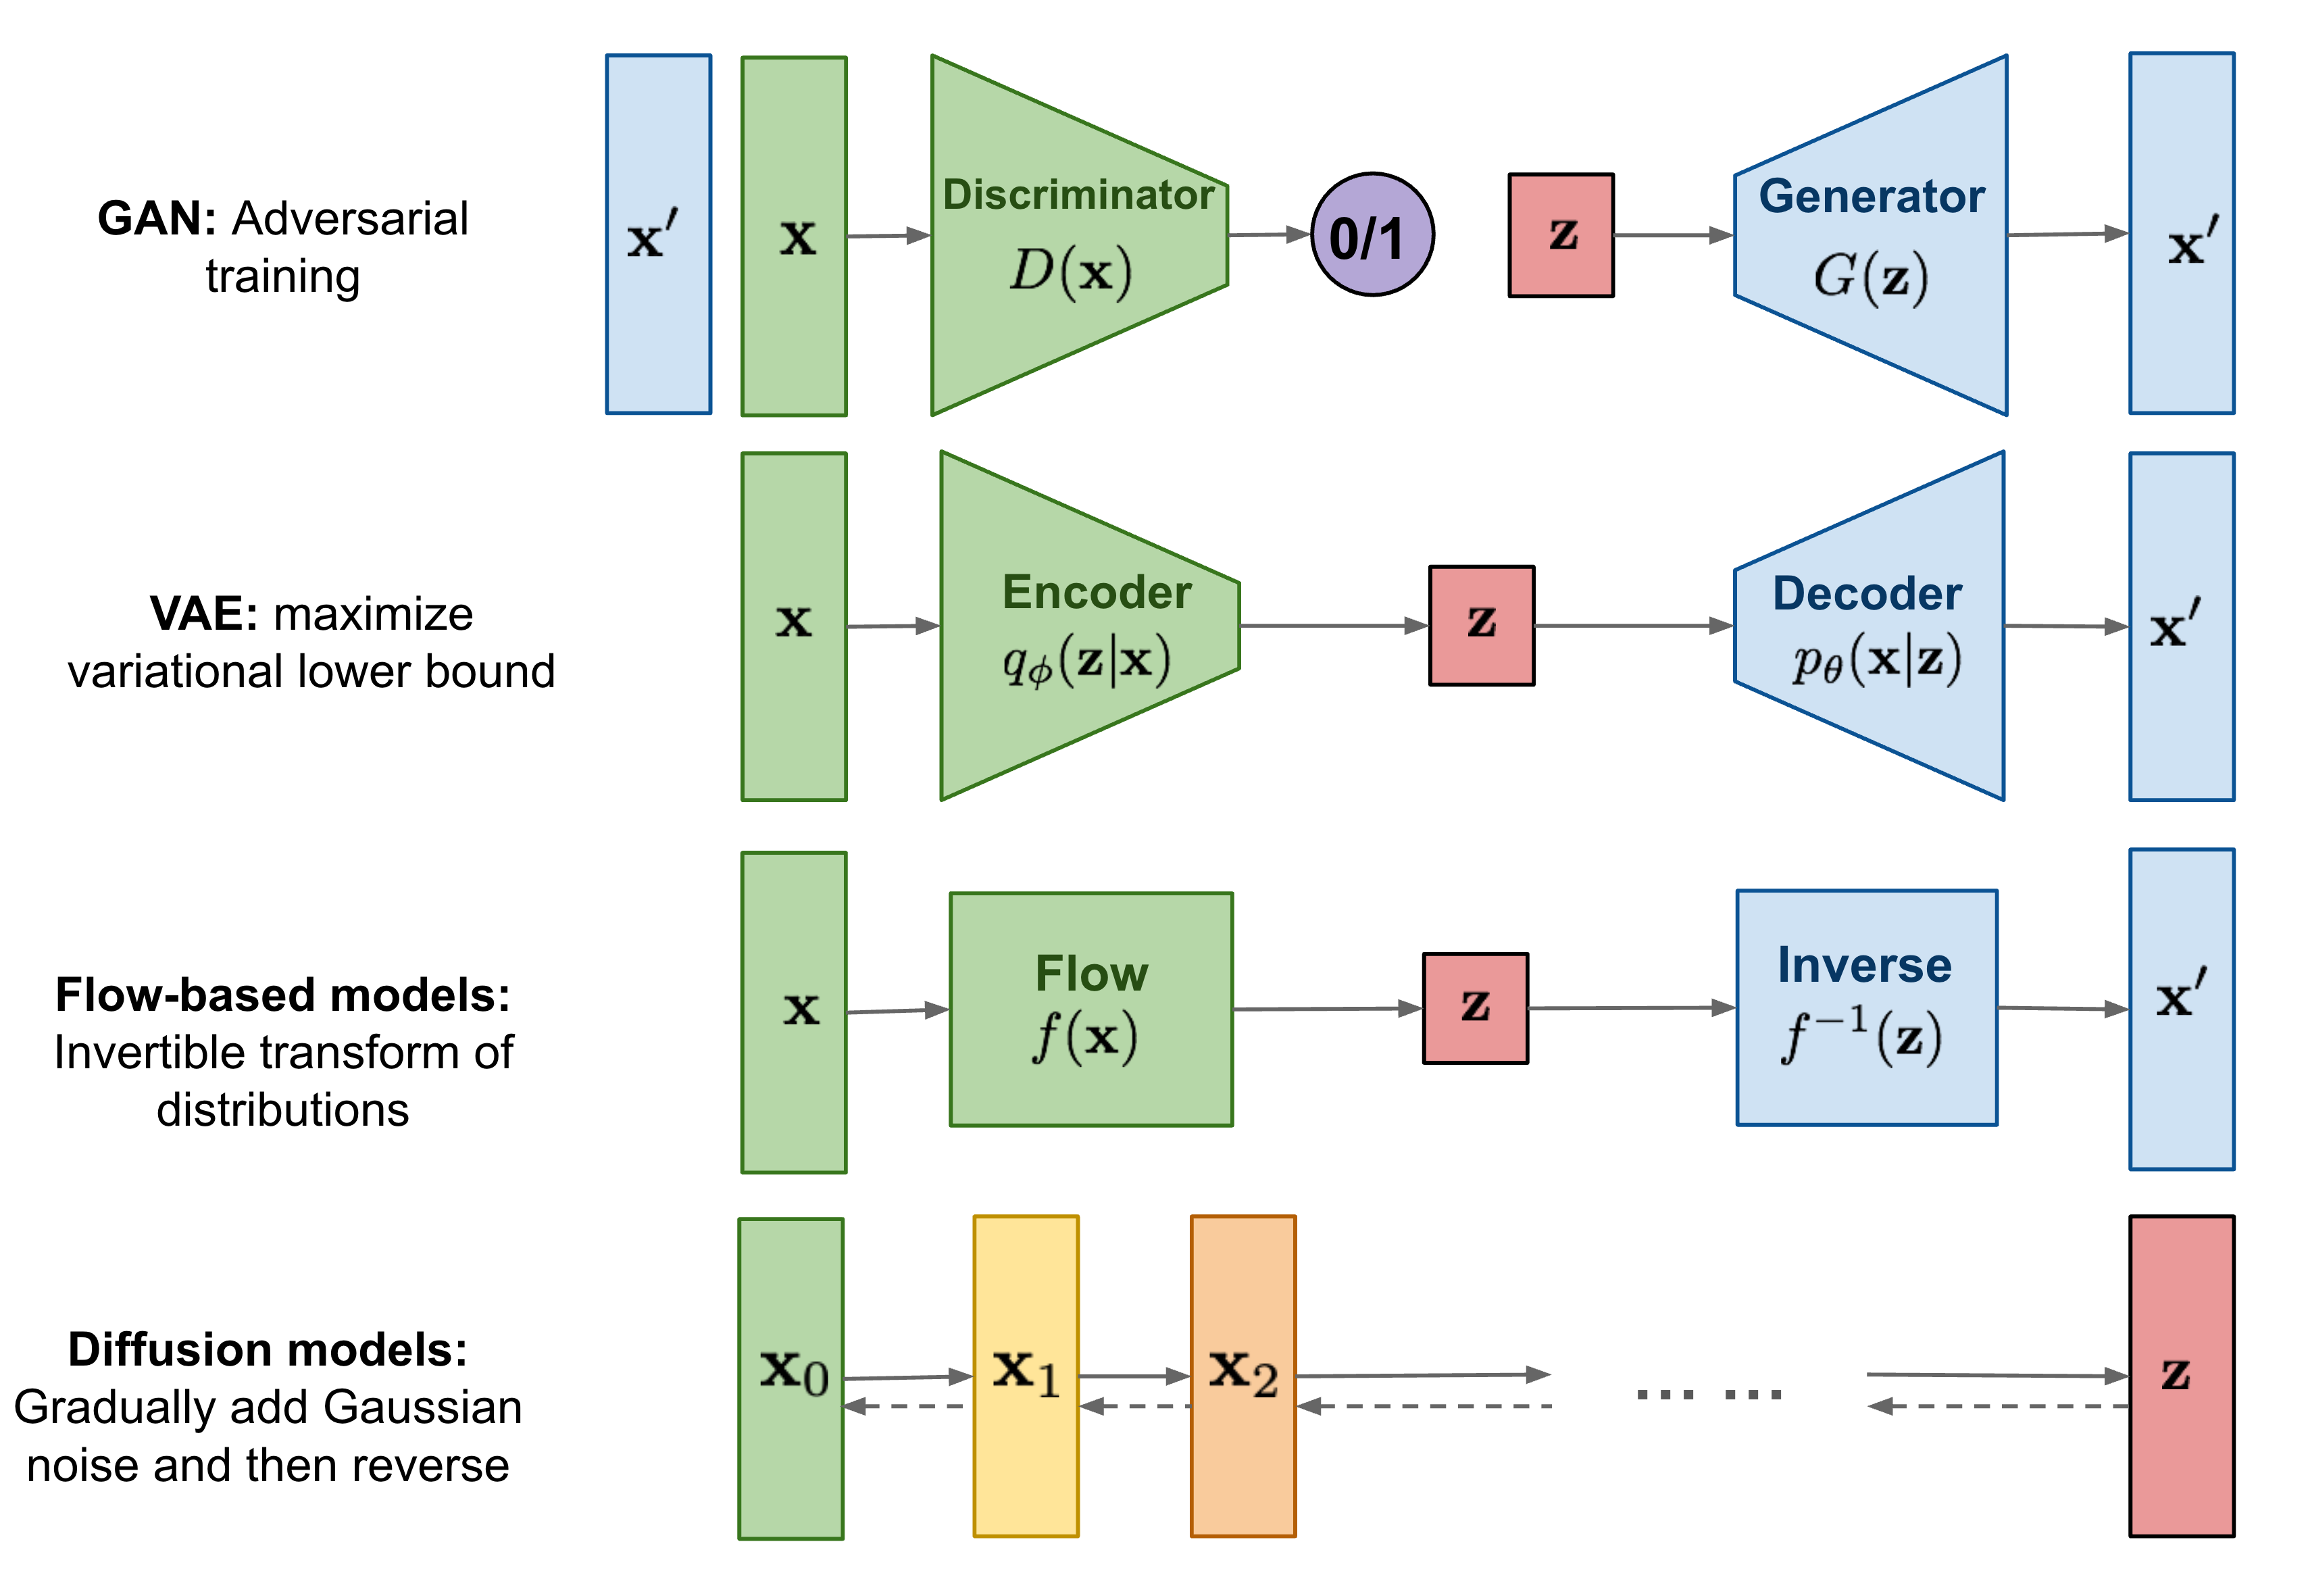
\includegraphics[width=\linewidth]{figs/generative-overview}
	\end{figure}
	\myfootnotewithlink{https://lilianweng.github.io/posts/2021-07-11-diffusion-models/}{Weng L. What are Diffusion Models?, blog post, 2021}
\end{frame}
%=======
\begin{frame}{The worst course overview :)}
	\vspace{-0.3cm}
	\begin{figure}
		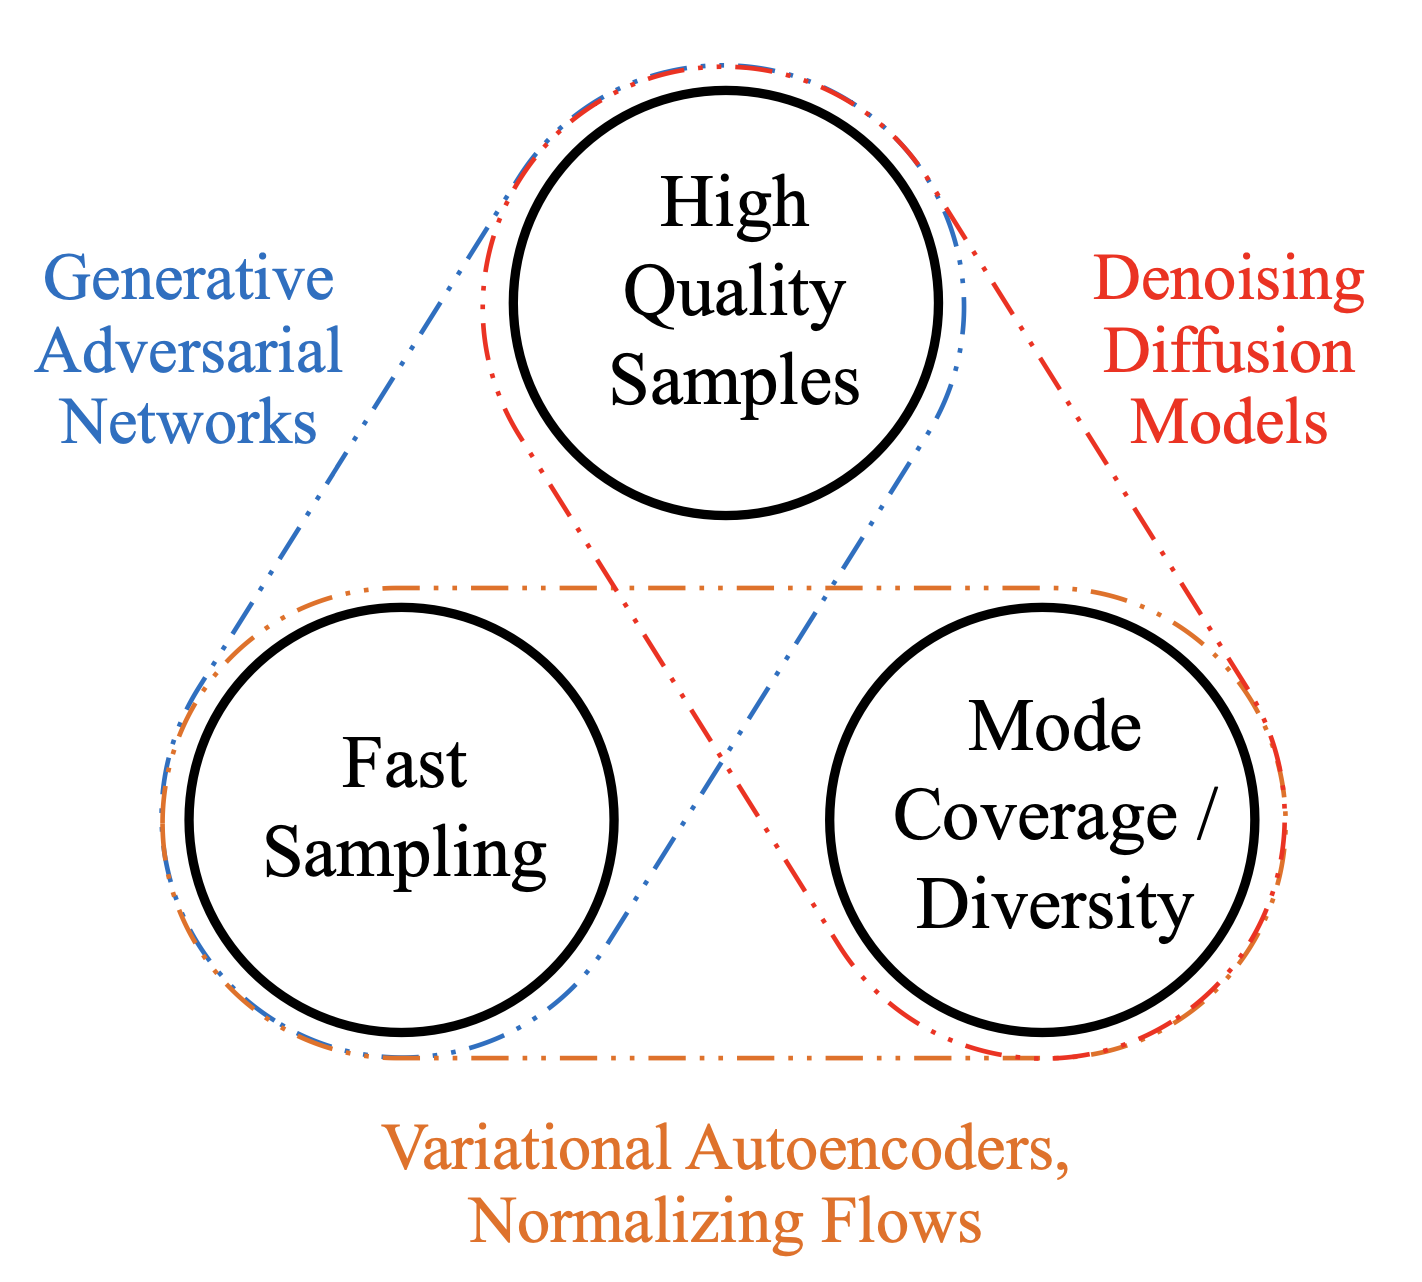
\includegraphics[width=0.45\linewidth]{figs/trilemma}
	\end{figure}
	\vspace{-0.5cm}
	\begin{figure}
		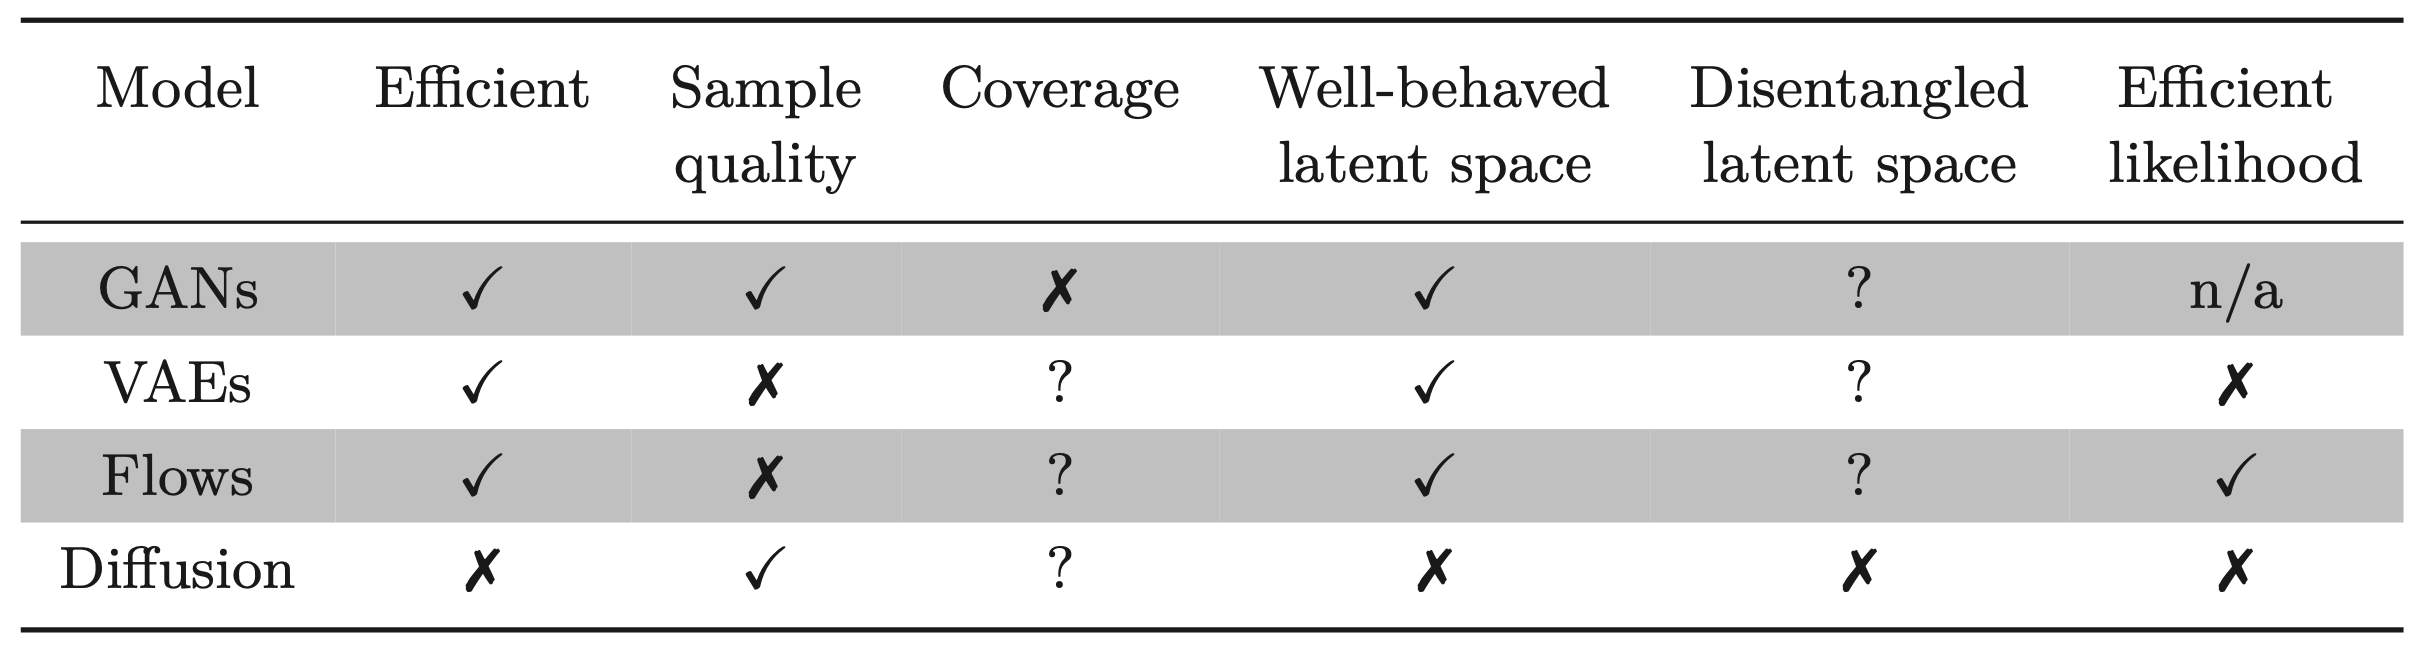
\includegraphics[width=0.9\linewidth]{figs/gen_comp_table}
	\end{figure}
	\myfootnote{\href{https://arxiv.org/abs/2112.07804}{Xiao Z., Kreis K., Vahdat A. Tackling the generative learning trilemma with denoising diffusion GANs, 2021} \\ \href{https://udlbook.github.io/udlbook/}{Simon J.D. Prince. Understanding Deep Learning, 2023}}
\end{frame}
%=======
\begin{frame}{Summary}
	\begin{itemize}
		\item Conical gaussian paths is the example of the effective FM technique.
		\vfill
		\item 
	\end{itemize}
\end{frame}
\end{document} 